\documentclass[11pt, oneside]{article}   	% use "amsart" instead of "article" for AMSLaTeX format
\usepackage[margin=0.7in]{geometry}                		% See geometry.pdf to learn the layout options. There are lots.
\geometry{letterpaper}                   		% ... or a4paper or a5paper or ... 
%\geometry{landscape}                		% Activate for rotated page geometry
%\usepackage[parfill]{parskip}    		% Activate to begin paragraphs with an empty line rather than an indent
\usepackage{graphicx}				% Use pdf, png, jpg, or eps§ with pdflatex; use eps in DVI mode
								% TeX will automatically convert eps --> pdf in pdflatex		
\usepackage{amssymb}
\usepackage{amsmath}
\usepackage{amsfonts}
\usepackage{booktabs}
\usepackage{listings}
\usepackage{dsfont}
\usepackage{wasysym}

\newcommand{\Var}{\mathrm{Var}}


\title{Determination of power profile and orificing for the 3500 MWth B\&B core}
\author{Chris Keckler}
%\date{}							% Activate to display a given date or no date

\begin{document}
\maketitle

It has been decided in agreement with the ANL co-PI that the second core which will be examined with respect to ARC system performance is a large 3500 MWth B\&B reactor designed by Qvist et al. \cite{Qvist_3D}.
In \cite{Qvist_3D}, this core has been modeled with r-z cylindrical transport models using the Serpent monte carlo code \cite{serpent}.
However, in order to perform safety analysis studies with SAS4A/SASSYS-1 \cite{SAS}, the power production within each assembly is required, and this cannot be extracted from a simple r-z model.
Furthermore, realistic flowrates for each channel need to be determined so that the assemblies can be properly cooled throughout the burn cycle, which requires the determination of orifice groups and flowrates.
In order to obtain these details, the r-z transport model of the core has been converted into a model with explicit hexagonal assembly geometry.
Once this model is successfully run, the results are fed into a newly devised optimization code to determine the orifice grouping and flowrates within each channel.
The work to accomplish these tasks is outlined in this document.

%%%%%%%%%%%%%%%%%%%%%%%%%%%%%%%%%%%%%%%%%%%%%%%%%%%%%%%%%%%%%%%%%%%%%%%
\section{Conversion to hexagonal geometry}

All previous modeling of the 3500 MWth core has utilized a simplified r-z cylinder geometry to save on both computational effort and the time that it takes to create the core layout in hexagonal geometry.
Each fuel batch is represented as an annular cylinder that preserves the volume and approximate location of the assemblies which it is meant to represent.
It has been shown in previous studies that, due to the relatively low probability of neutron interaction and resulting long mean free paths in a fast spectrum system, this type of spatial approximation is justifiable and does not introduce a significant error into the overall results \cite{heidet_thesis}.
Additionally, this sort of approximation allows the reactor geometry to be treated as a continuum, which avoids issues with specific assembly orientation and positioning and allows for rapid, simple changes to be made in the design during the initial scoping phase.
This approximation is one of the key reasons why codes such as ADOPT \cite{ADOPT} can be effectively used.

Now that more detailed studies of this core are desired, however, a more accurate model is necessary.
For this reason, the cylinder model is converted to a hexagonal lattice.
Each lattice position consists of a homogeneous material that represents the proper isotopics of each batch smeared across the batch volume at nine separate axial levels.
Therefore, each assembly within a given batch has the same composition at BOC, regardless of its location within the core.
Because all assemblies for a given batch are located very close to each other, the error resulting from this approximation is assumed to be minor, although it is not explicitly quantified here.
Furthermore, the cost to achieve a more accurate material distribution in for each assembly would be high, as an additional equilibrium cycle calculation performed with a code such as MocDown \cite{mocdown} would need to be performed.

To begin the process of converting to hexagonal geometry, the number of assemblies per fuel batch is determined by dividing the batch volume by the design assembly volume.
Doing this indicates that each batch should have 41 assemblies. 
Additionally, the preliminary design specifies that there are 19 control rod assemblies and 12 batches.
With these parameters, the process of creating a hexagonal lattice proceeds largely by trial and error.
The goals guiding the lattice creation is to maintain azimuthal symmetry of the core while keeping all of the assemblies for a given batch bunched together within a limited number of rings.

The desire for symmetry does not work well with 41 assemblies per batch, as the number of positions within a given ring of a hexagonal lattice is even.
After many attempts to obtain a suitable core layout with 41 assemblies per batch, the decision was made to instead use 42 assemblies per batch. 
Although this introduces additional fuel into the design, only 12 assemblies are added, in comparison to the 492 assemblies already in the design.
In addition, due to the nature of B\&B cores, only a few of those additional 12 assemblies are producing appreciable power during a given burn cycle.
Therefore, the impact of the additional assemblies is assumed to be minor, although this has not been quantified explicitly.

The final core layout settled on is depicted in Figure \ref{fig:BnB_layout}, where the batches are labeled with numbers 1-12.
This core has 1/6 azimuthal symmetry and 18 control assemblies laid out in a ring, with a 19th control assembly placed in the central position.
A ring of reflector assemblies surround the outermost blanket assemblies, with an additional ring of shields surrounding that.
This core design is suitable for the in-bounce-out shuffling scheme that this core utilizes, as it has the same number of assemblies in each batch and the batches generally are in concentric rings, allowing fuel to be moved consistently and progressively both inwards and outwards.

\begin{figure}[h!]
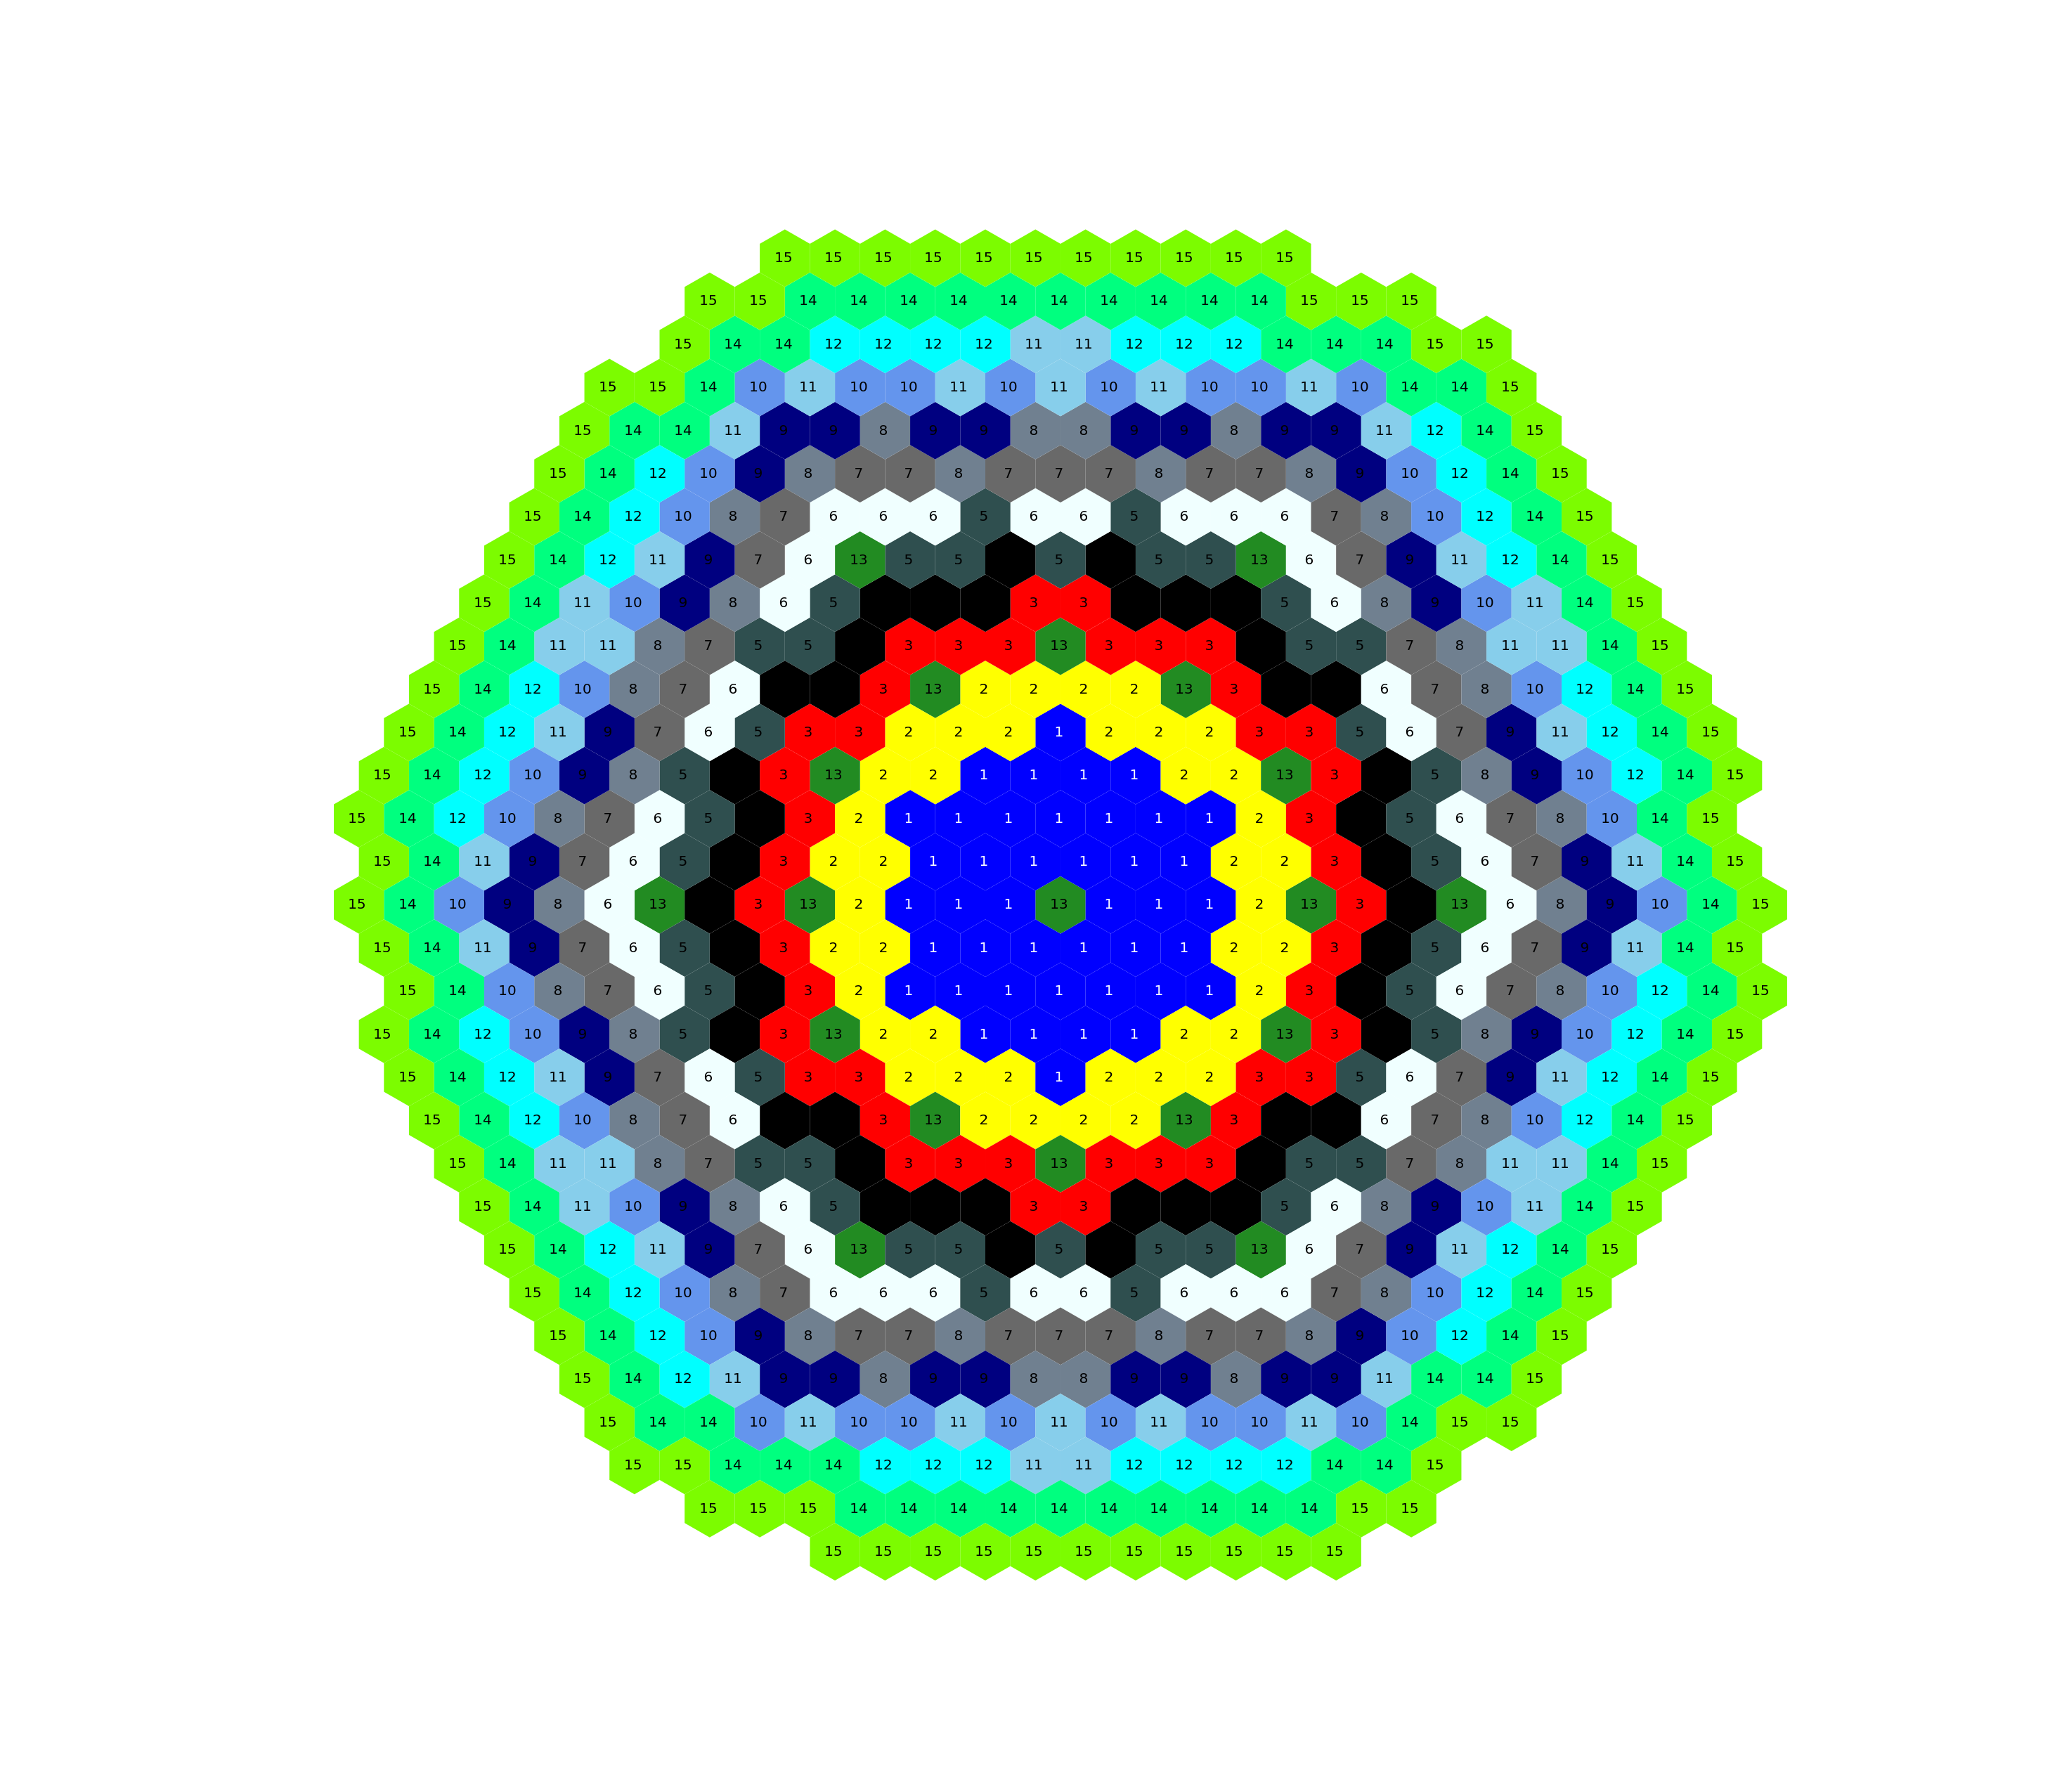
\includegraphics[width=18cm]{BnB_layout}
\centering
\caption{Core layout of the 3500 MWth B\&B core transport model depicting the locations of each batch and control assemblies.}
\label{fig:BnB_layout}
\end{figure}

%%%%%%%%%%%%%%%%%%%%%%%%%%%%%%%%%%%%%%%%%%%%%%%%%%%%%%%%%%%%%%%%%%%%%%%
\section{Power profile and reactor characteristics}

Once the core layout was specified, the model was run with Serpent2 to obtain the power profile on an assembly basis.
This is done by utilizing the mesh-tally functionality of the code.
Because power production via gamma heating in control and reflector assemblies (and additionally fuel assemblies towards the radial periphery) is important for safety analysis, it is desirable to include gamma transport within the calculation.
This is accomplished simply by using the newly developed coupled neutron-gamma transport capability within Serpent2 version 2.1.29, which requires only a few extra lines added to the input.
For these calculations, the ENDF/B-VII \cite{endf} and MCPLIB84 \cite{mcplib} cross section libraries are used for neutron and photon transport, respectively.

Initially, there were issues with fission source convergence that caused power profiles to be skewed towards particular sides of the geometry, as depicted in Figure \ref{fig:skewed_profile}.
This power skew convergence issue results from the shuffling scheme which is employed in this core design.
As fuel is introduced to the radial periphery, it is shuffled inwards a few times as it accumulates burnup and breeds Pu-239.
After a few inward shuffles, the fuel then skips a few rings and is placed in the core center, where it is further shuffled outwards into the radial middle. 
This in-bounce-out shuffle scheme causes most of the power production to be in an annular region towards the radial middle of the core.
The central core region is then composed of mostly fertile U-238, which predominantly absorbs neutrons and acts somewhat like a central shield.
This makes the core very loosely azimuthally coupled, which presents a challenge to monte carlo analysis.
Although this issue was likely present in the r-z modeling of the same core, it was likely never discovered because the tallies only captured the power profile averaged over the batch annuli.

\begin{figure}[h!]
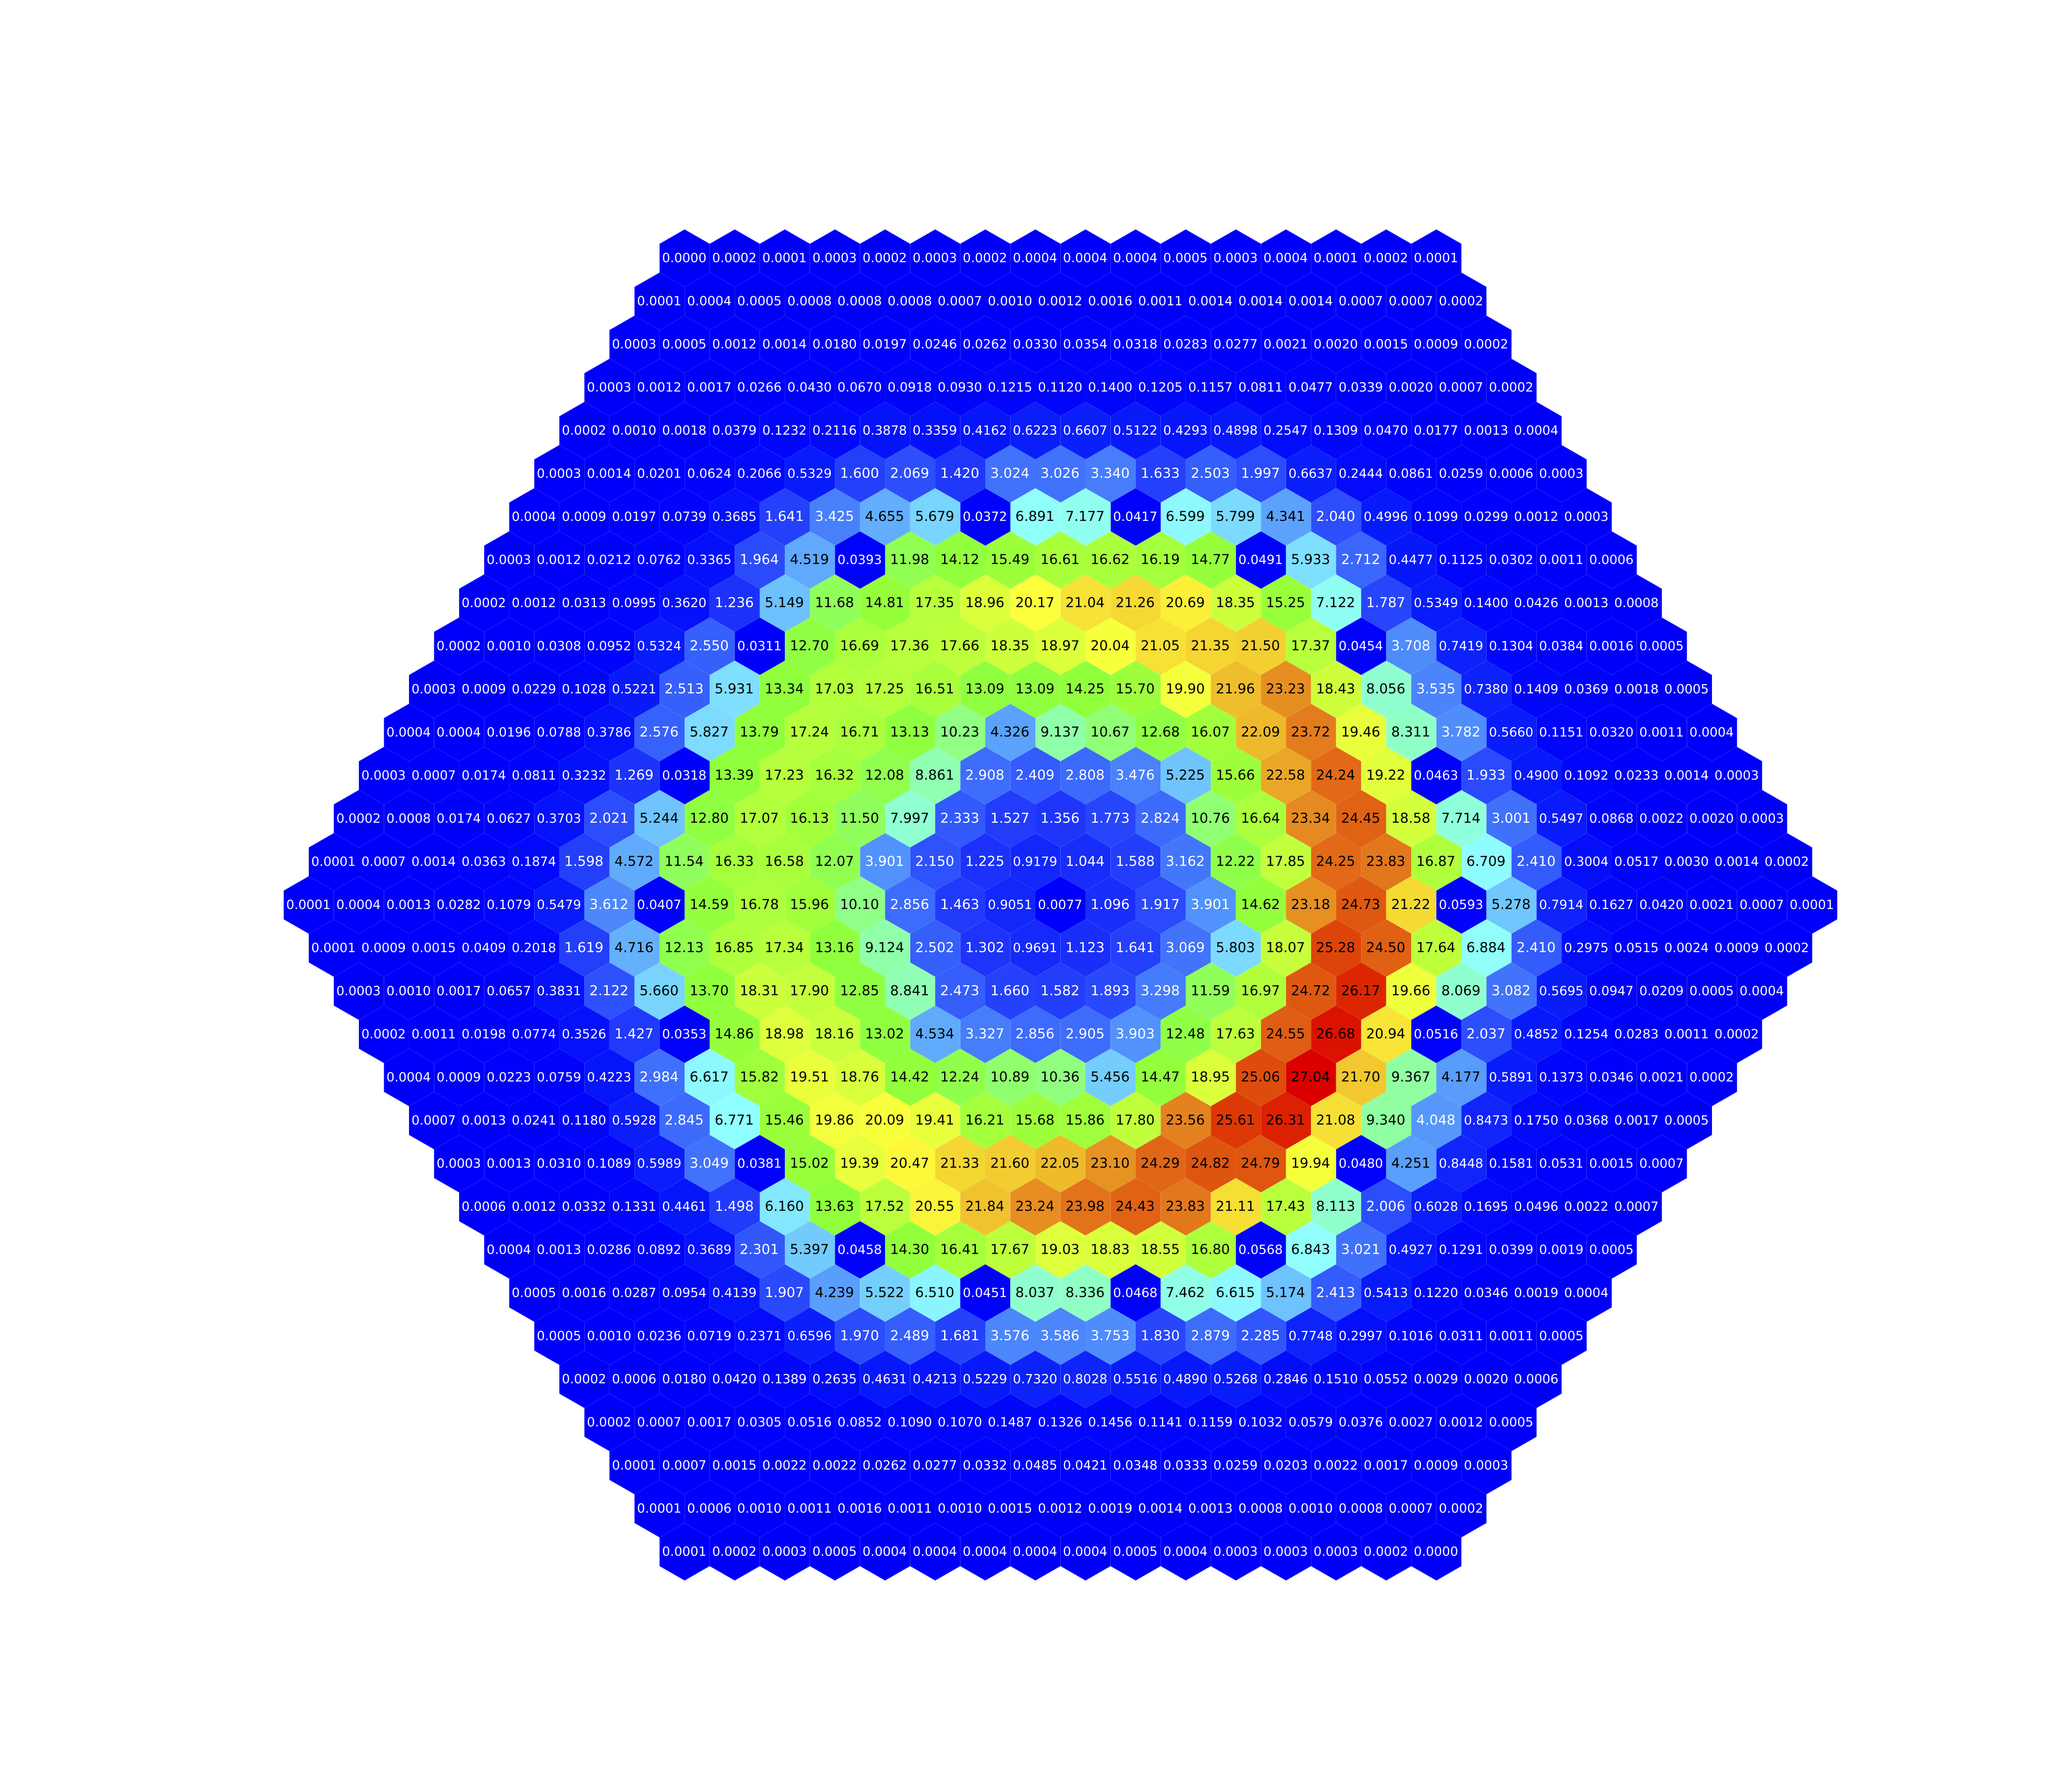
\includegraphics[width=16cm]{skewed_profile}
\centering
\caption{Example of a power profile resulting from a simulation with a non-converged fission source.}
\label{fig:skewed_profile}
\end{figure}

With the hexagonal geometry, this convergence issue was discovered early on in the process, and considerable time was spent performing a convergence study to determine how many particles are needed to obtain proper statistics.
Because the core is 1/6 symmetric, it is easy to judge whether the monte carlo calculation is converged by simply seeing if the power profile is also 1/6 symmetric.
Additionally, a plot of the norm of the error in the power profile vector versus the number of particles used in the simulation is shown in Figure \ref{fig:norm}, where the "exact" solution is taken to be the results from the 600,000 particle simulation.

\begin{figure}[h!]
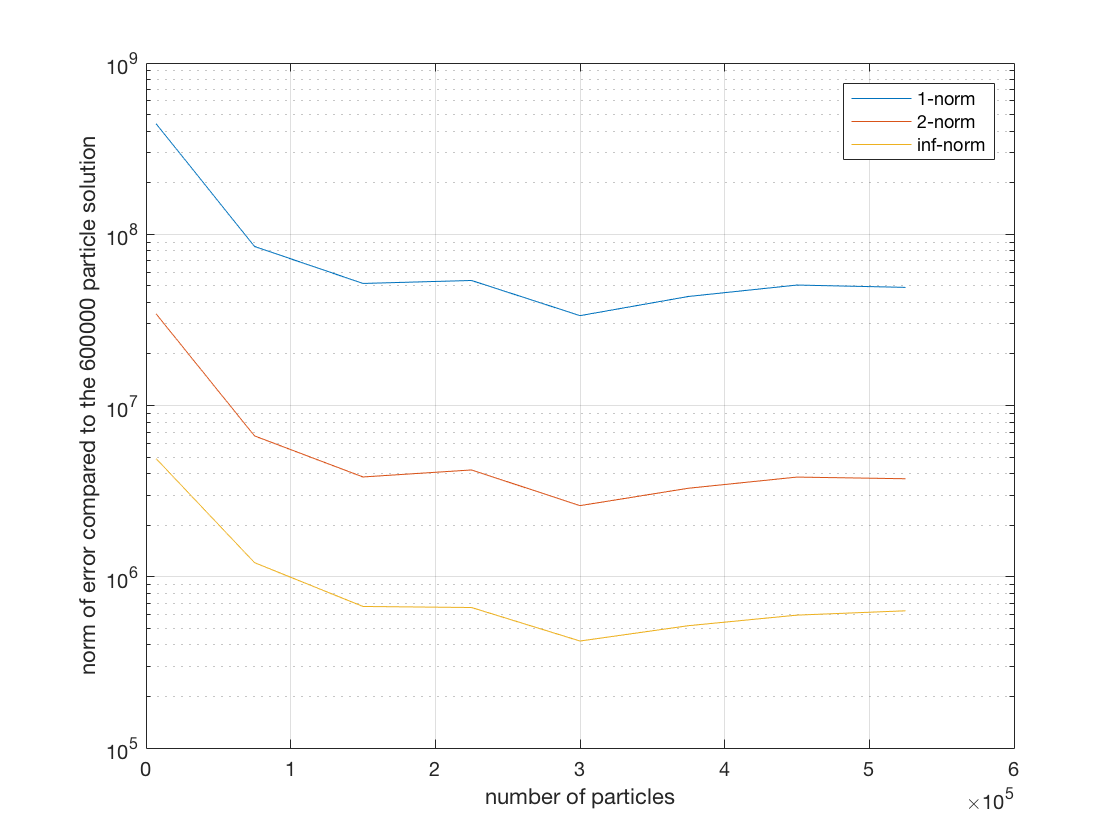
\includegraphics[width=10cm]{norm}
\centering
\caption{Norm of the error in power profile calculated with Serpent2 as compared against the solution with 600,000 particles per cycle.}
\label{fig:norm}
\end{figure}

From Figure \ref{fig:norm}, it may be judged that the solution is converged at near 300,000 particles, but it should be noted that statistical error and the random number seed for the monte carlo calculations plays a large role in the error determination. 
When observing the power profile with 300,000 particles, it is seen that the expected 1/6 symmetry is not quite achieved, and so it is judged that this solution is not yet converged.
However clearly the solution is converged by using 600,000 particles, and this is therefore the conservative estimate used for the remaining calculations.
This is a considerable amount, and requires a large computational effort for each burn step, especially when using the coupled neutron-photon transport mode.

Once this was determined, a full coupled neutron-gamma transport calculation with burnup over the cycle was performed.
The two year burn cycle was divided into 4 equal-length steps to later examine how the power profile changes over the cycle, as this can be substantial in B\&B designs.
The results of these calculations are presented in Figures \ref{fig:BnB_0}-\ref{fig:BnB_3}.

\begin{figure}[h!]
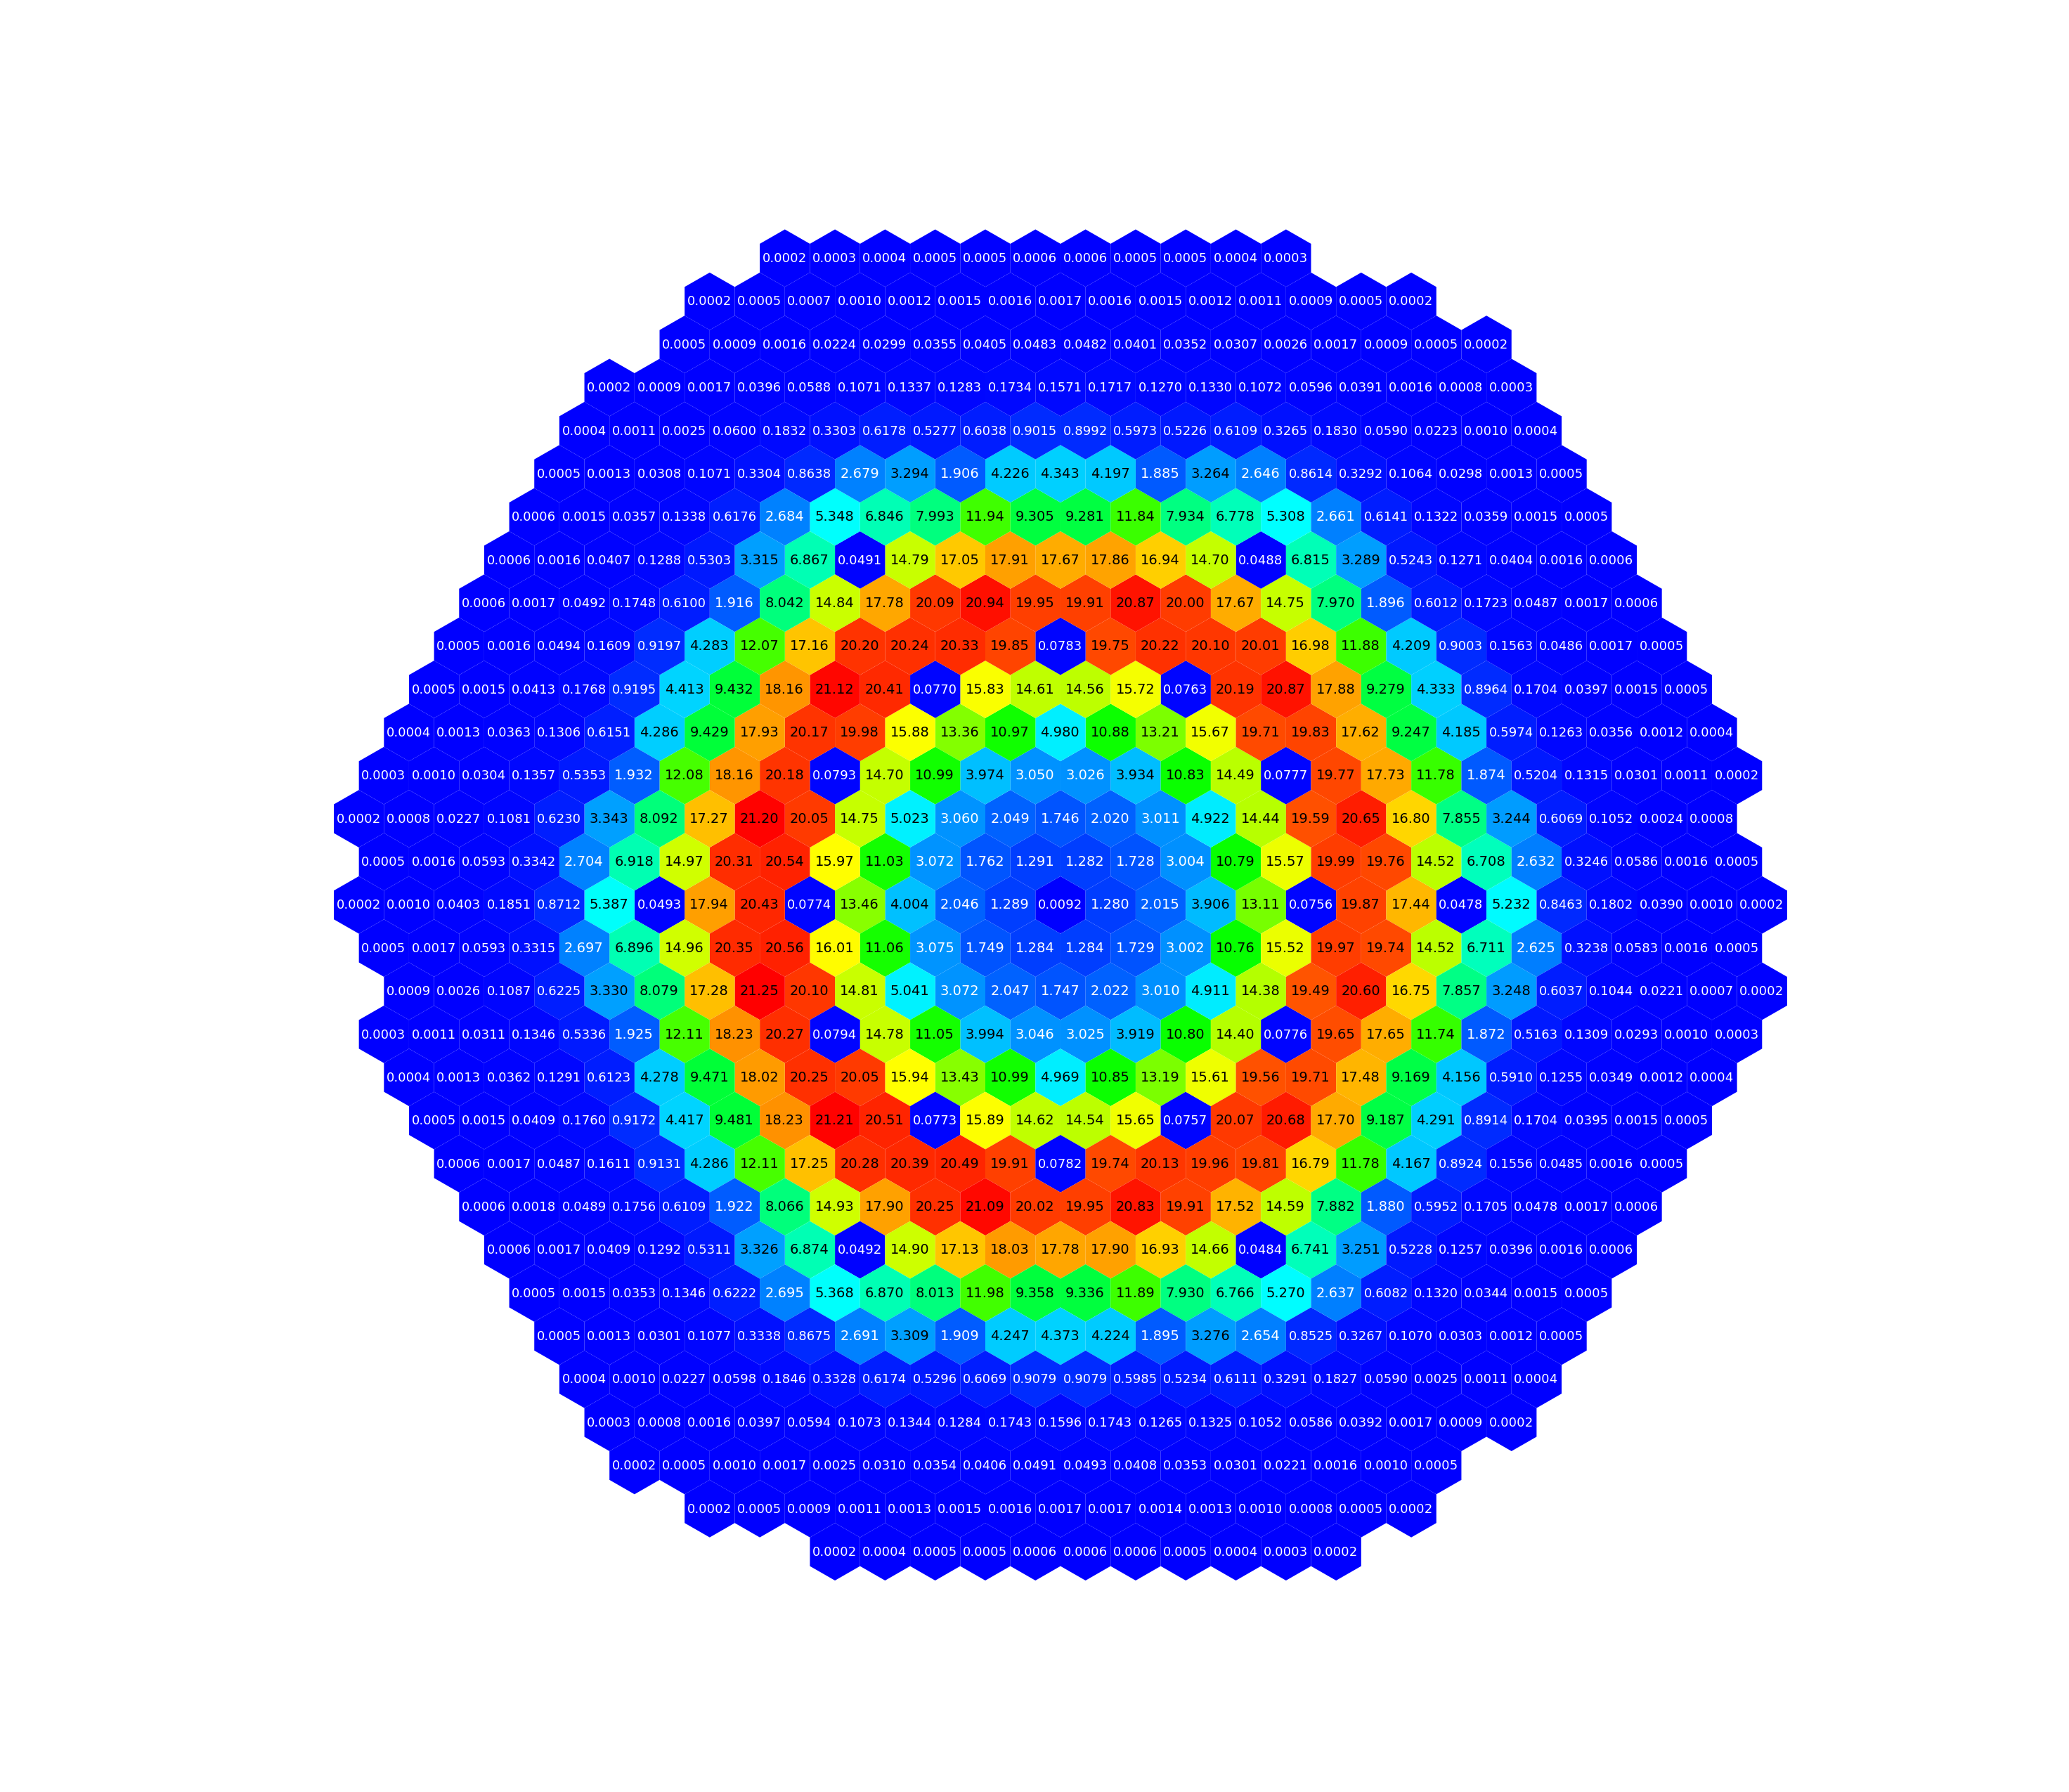
\includegraphics[width=16cm]{BnB_0}
\centering
\caption{Converged power profile of the 3500 MWth B\&B core at BOEC. Depicted powers are in axially integrated and listed in MW.}
\label{fig:BnB_0}
\end{figure}

\begin{figure}[h!]
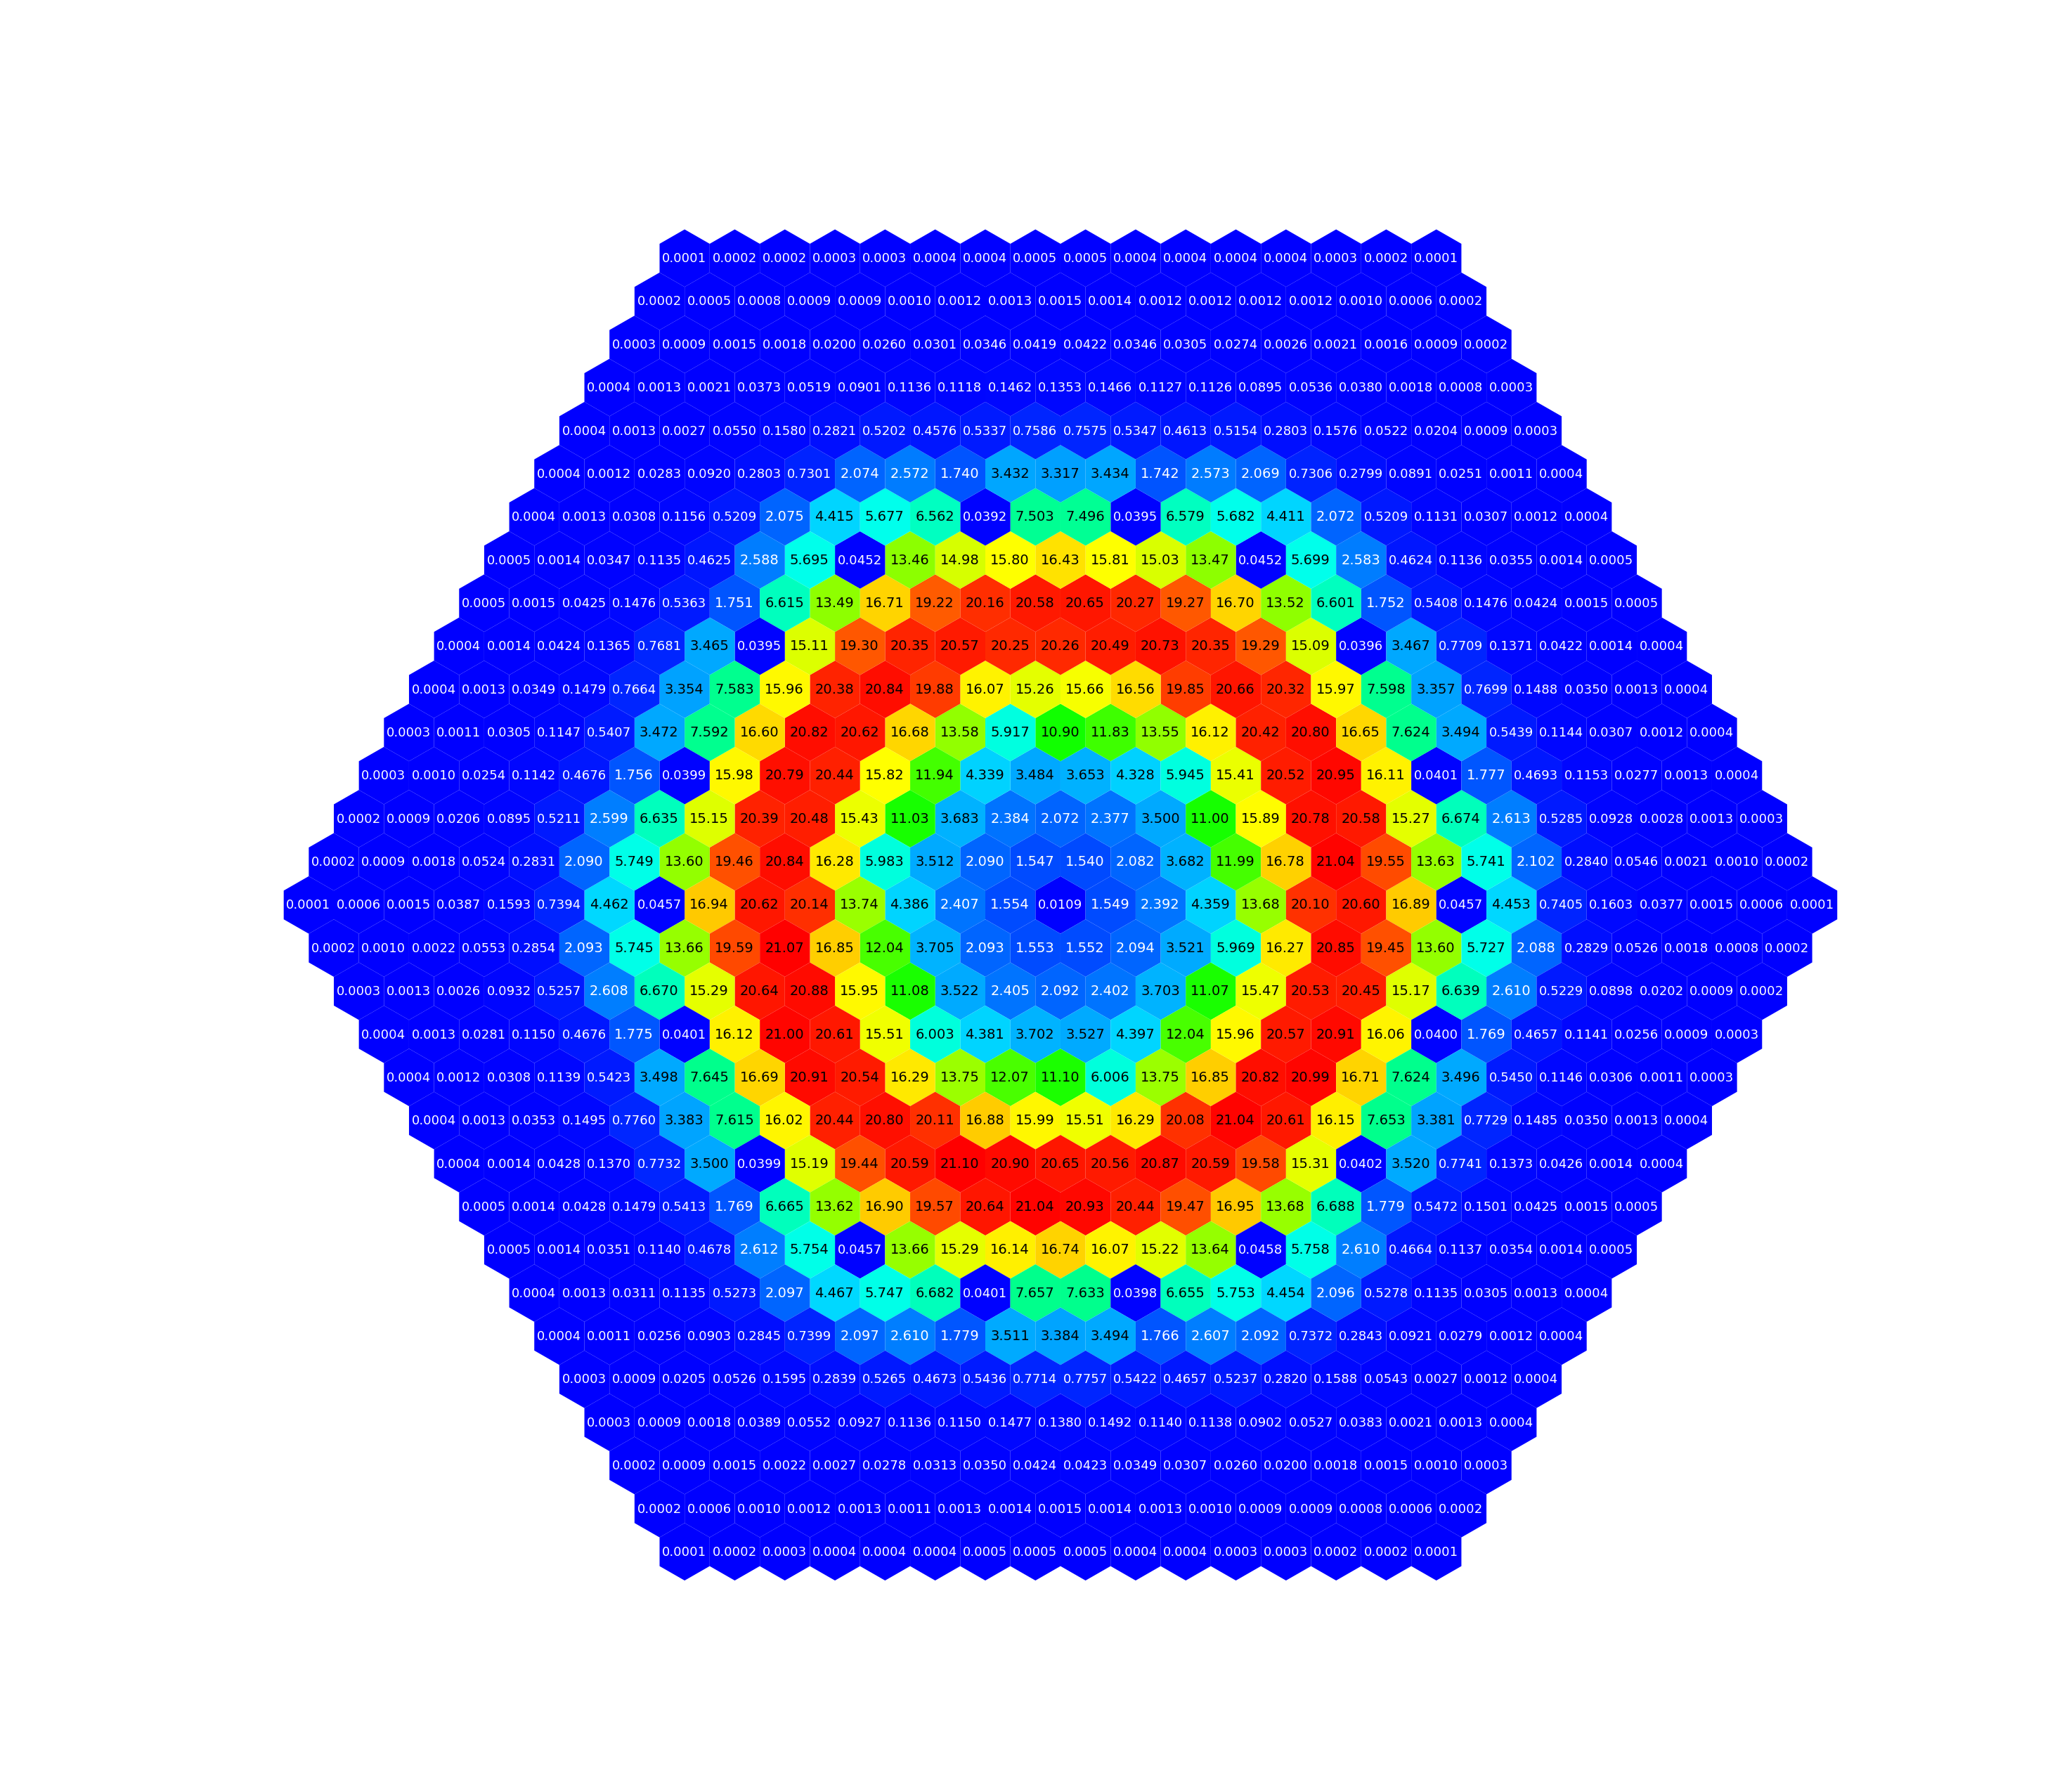
\includegraphics[width=16cm]{BnB_1}
\centering
\caption{Converged power profile of the 3500 MWth B\&B core at MOEC1. Depicted powers are in axially integrated and listed in MW.}
\label{fig:BnB_1}
\end{figure}

\begin{figure}[h!]
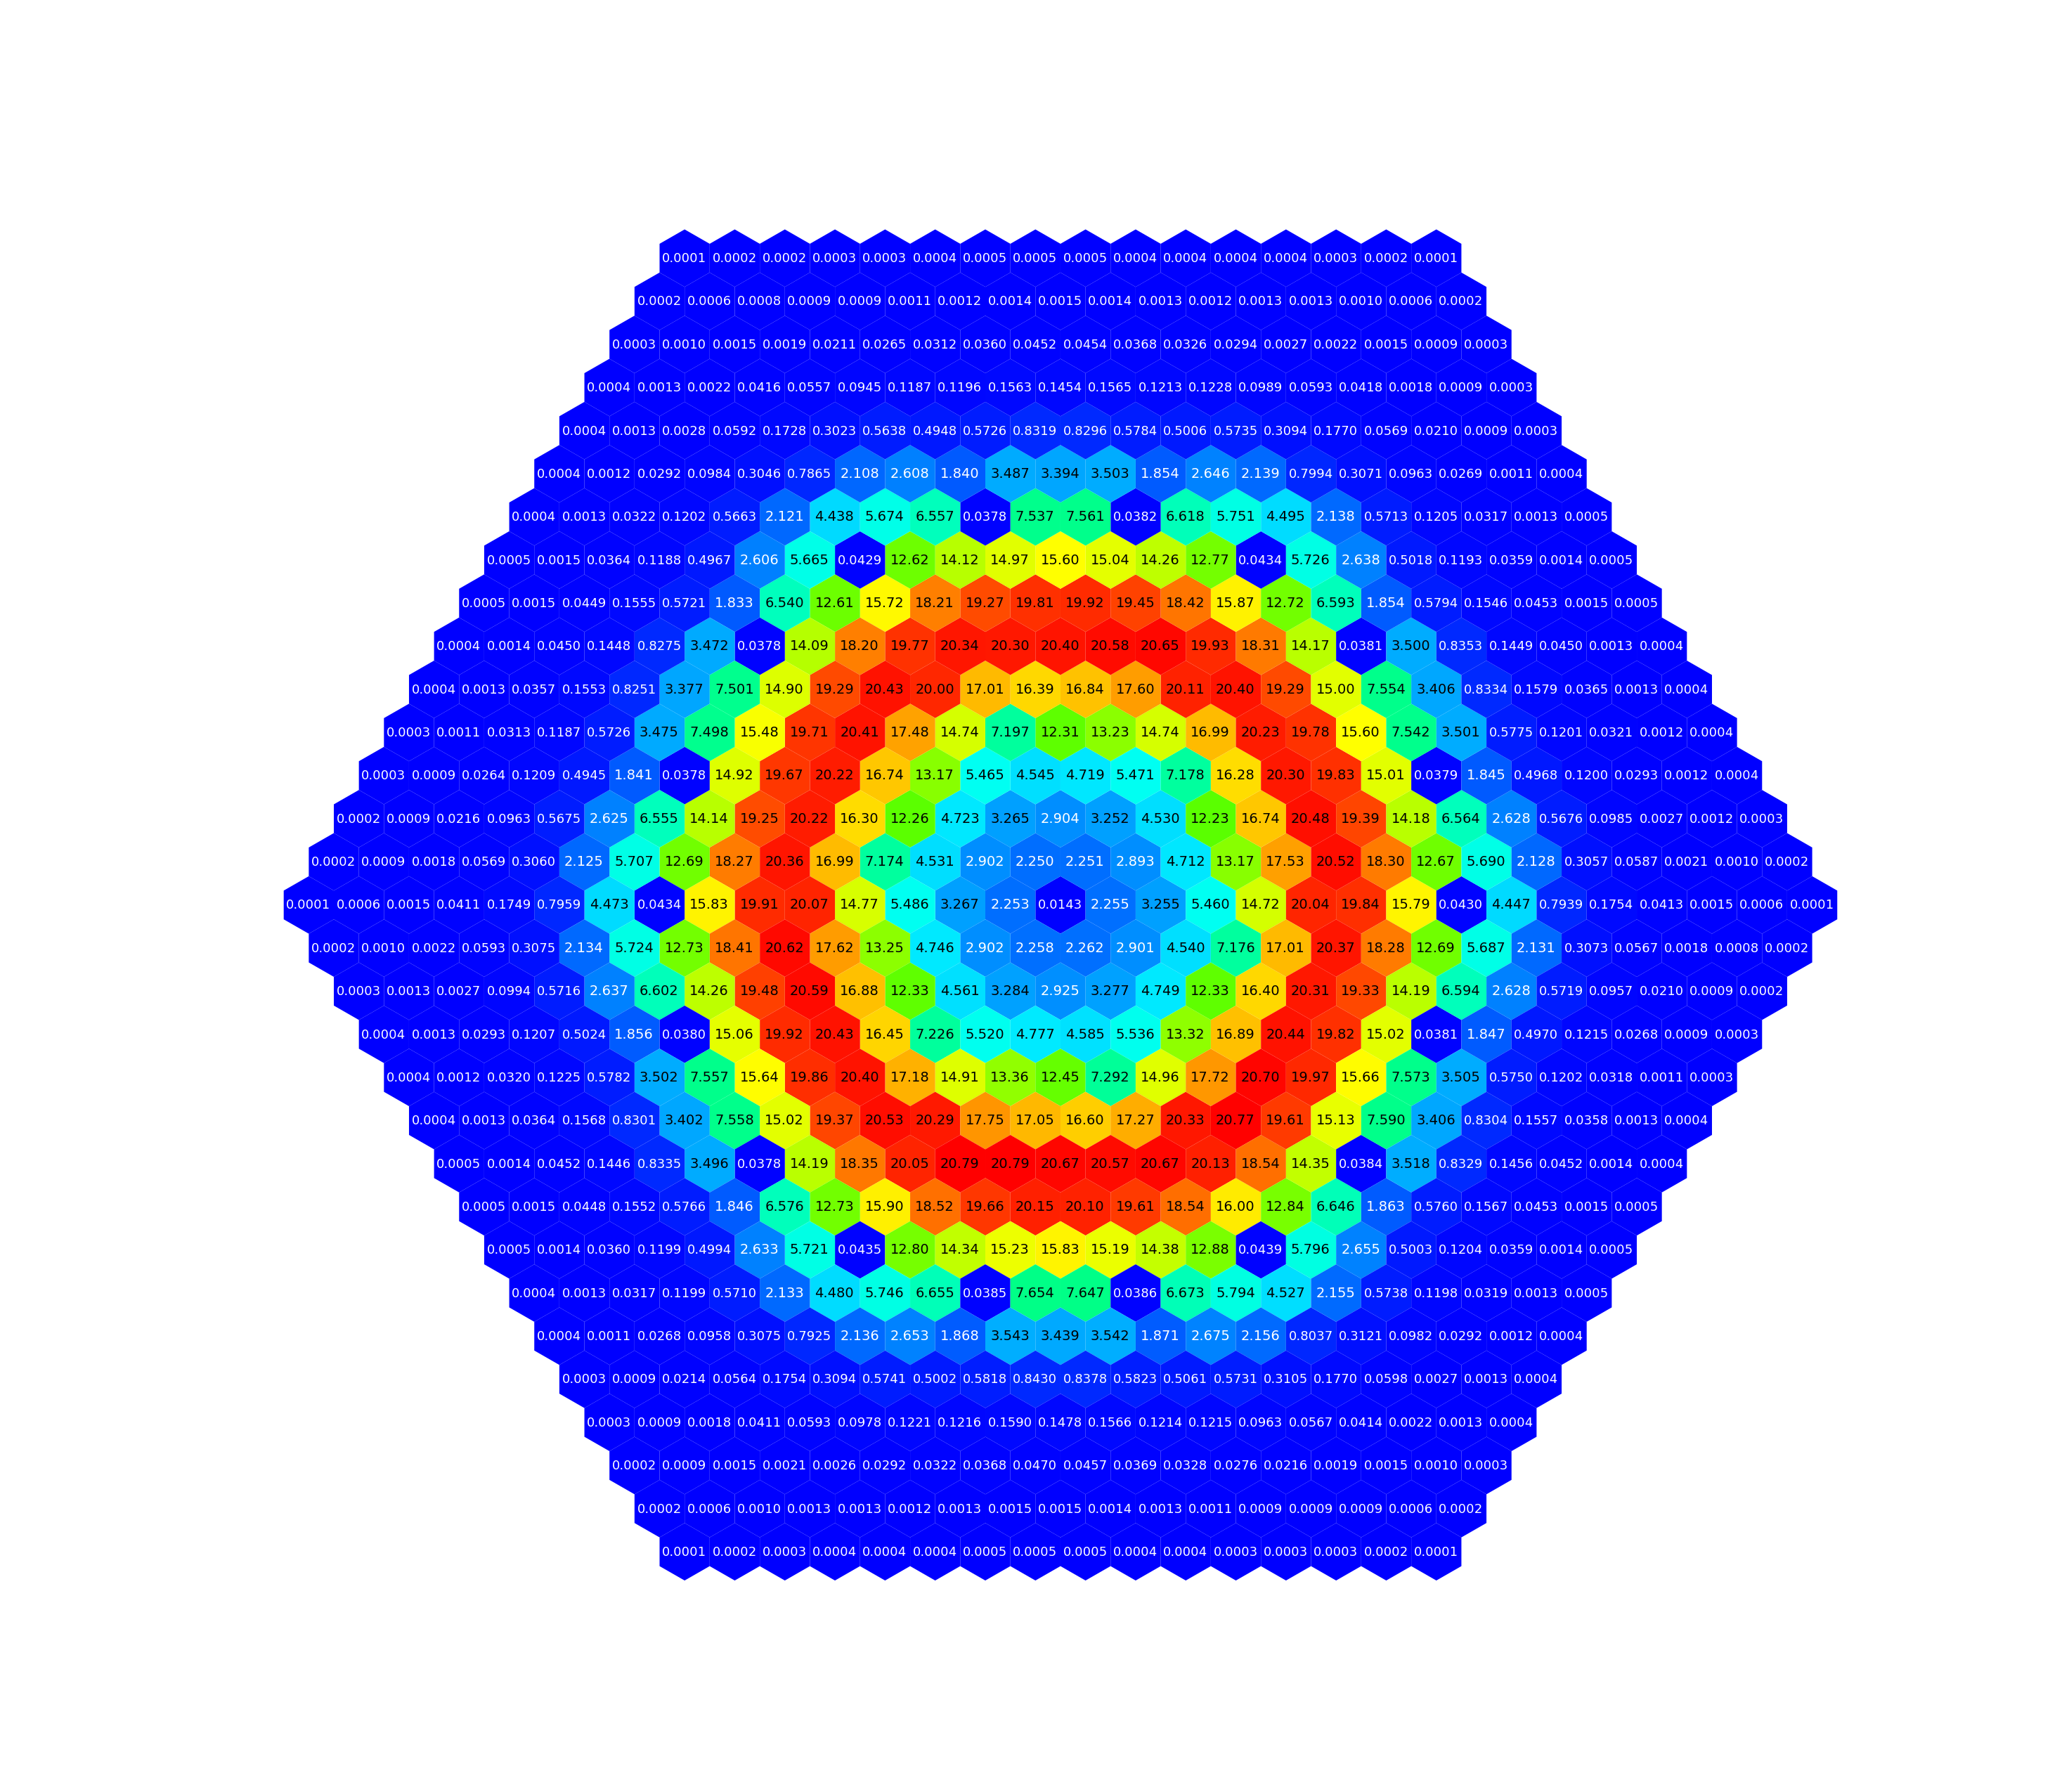
\includegraphics[width=16cm]{BnB_2}
\centering
\caption{Converged power profile of the 3500 MWth B\&B core at MOEC2. Depicted powers are in axially integrated and listed in MW.}
\label{fig:BnB_2}
\end{figure}

\begin{figure}[h!]
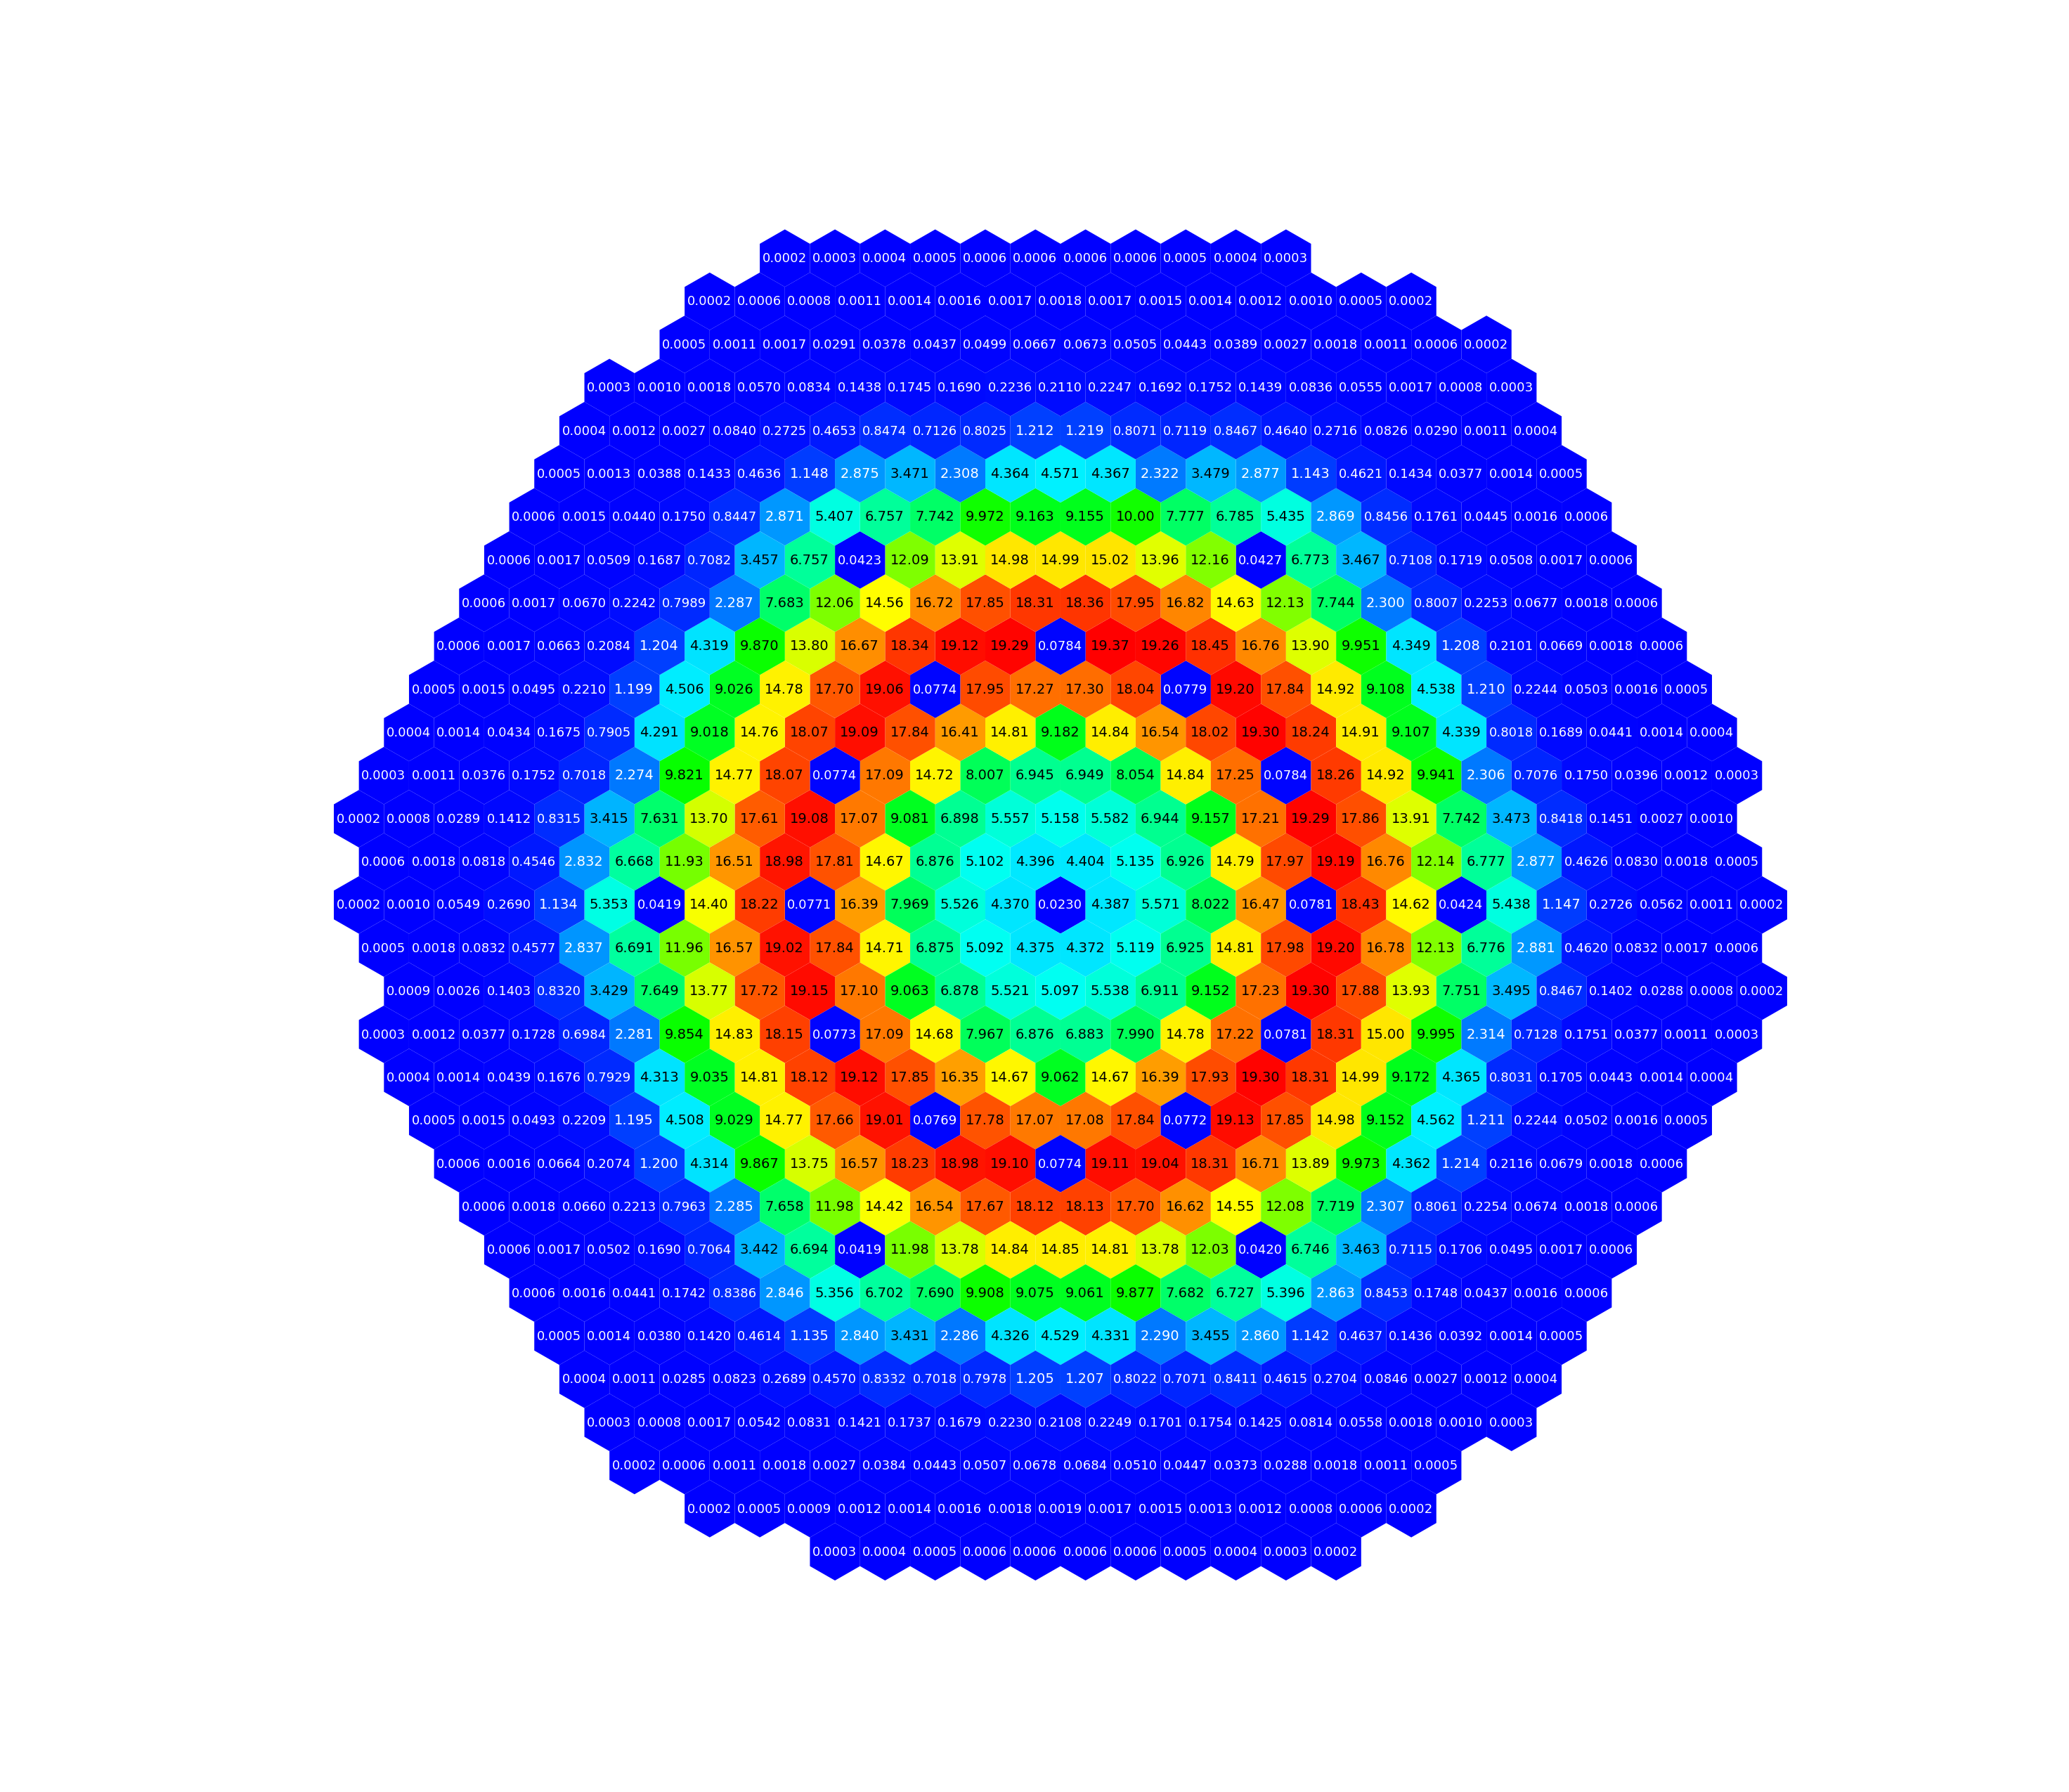
\includegraphics[width=16cm]{BnB_3}
\centering
\caption{Converged power profile of the 3500 MWth B\&B core at EOEC. Depicted powers are in axially integrated and listed in MW.}
\label{fig:BnB_3}
\end{figure}

From Figures \ref{fig:BnB_0}-\ref{fig:BnB_3}, it can be seen that the power production at BOEC mainly takes place in a very well-defined annulus, but as the cycle progresses, the power production shifts inward towards the core center. 
This shift is partially quantified in Table \ref{tab:power_profile} as $\Delta P_{max}$, the maximum power change within an assembly between burn steps.
Throughout the entire equilibrium cycle, the largest power shift within an assembly is 3.95 MW.

\begin{table}[]
\centering
\caption{Aspects of the power profile for each burn step in the equilibrium cycle of the 3500 MWth B\&B core.}
\label{tab:power_profile}
\begin{tabular}{@{}cccc@{}}
\toprule
Burn Step & Burn Time (days) & Radial Peaking Factor & $\Delta P_{max}$ (MW) \\ \midrule
BOEC      & 0                & 3.3                   &          -             \\
MOEC1     & 243.3            & 3.1                   & 1.40                  \\
MOEC2     & 486.6            & 3.1                   & 1.41                  \\
EOEC      & 730              & 3.0                   & 1.37                  \\ \bottomrule
\end{tabular}
\end{table}

The impact of gamma heating can be seen clearly in the control assemblies, which contain no fissionable material, but still manage to produce over 40 kW in some assemblies at various points in the cycle.
This is more than many of the outer blanket assemblies, and is clearly non-negligible for safety analysis.

Another striking aspect of the power profile is the number of fueled assemblies which produce very little power.
In total, the assemblies in batches 8-12 produce less than about 1\% of the power at each burn step, even though they account for 40\% of the total fuel in the core.
This important observation helps to understand why the orificing process can be so difficult in B\&B cores.
When an assembly is first placed into the core, it may produce exceedingly little power, but by the end of its residence in the core, it will be the primary power producer, with many megawatts of power being produced from just that single assembly.
This large power increase makes it difficult to design an orifice that can efficiently cool the assembly for its entire reactor residence time.

This same phenomenon causes the reported radial power peaking factors in Table \ref{tab:power_profile} to be somewhat misleading, as the concept of peaking factor implies a distribution of powers centered about some mean value.
Although the radial peaking factors are around 3 for the duration of the cycle, in actuality the power profile is quite bimodal, with a very large amount of assemblies at low powers in the kilowatt range and a smaller amount clustered at higher powers in the megawatt range. 
This bimodality is depicted in Figure \ref{fig:bimodality}, where the mean assembly power level at each burn step is ...

\begin{figure}[h!]
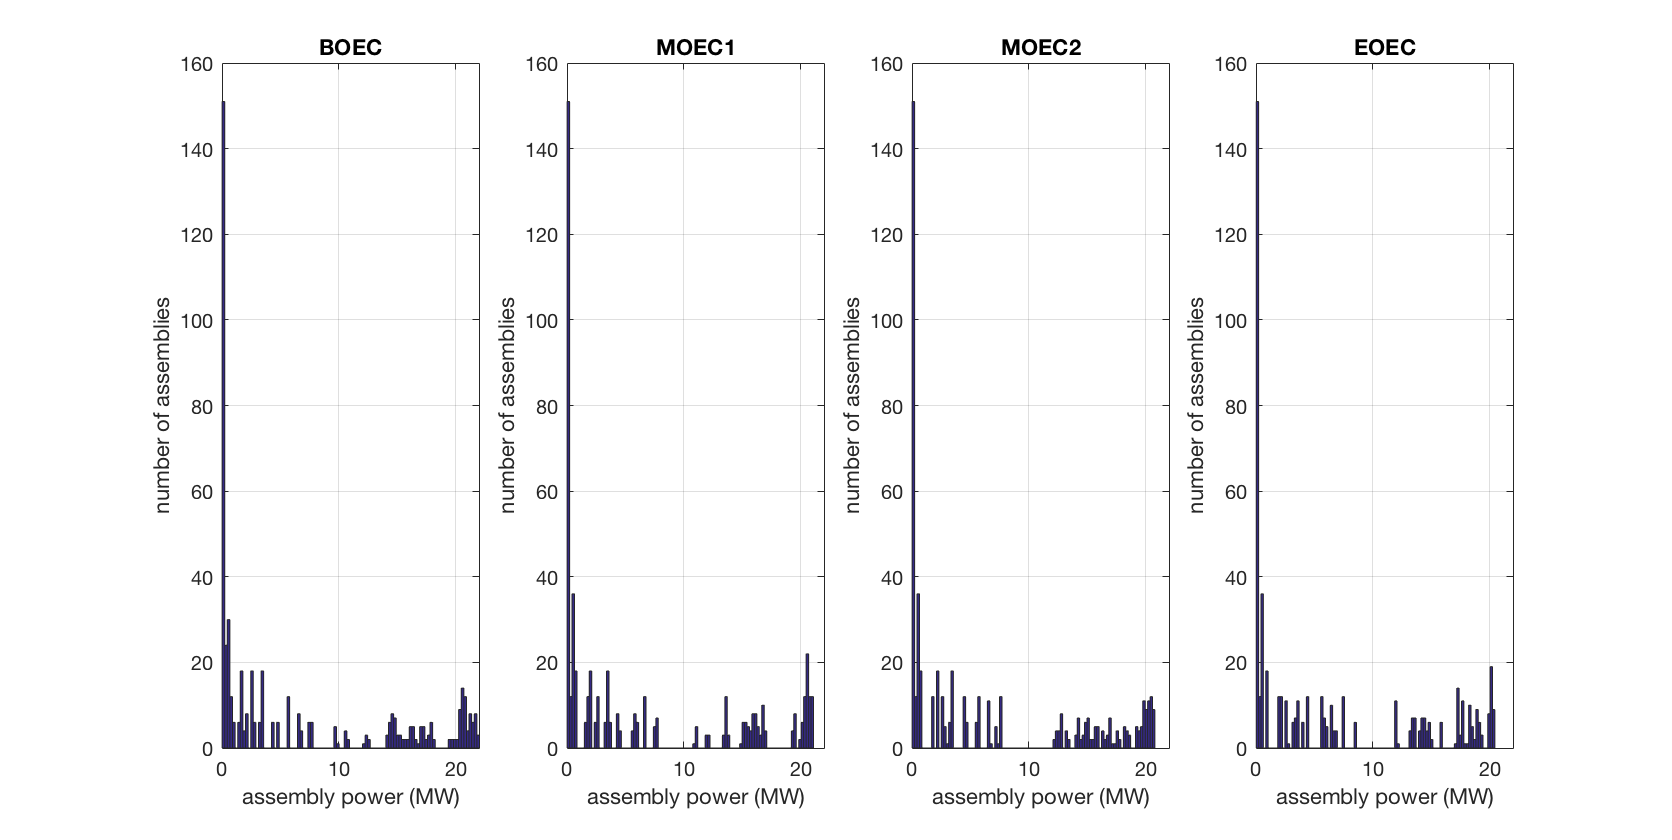
\includegraphics[width=18cm]{bimodality}
\centering
\caption{Histogram of assembly powers in each assembly of the 3500 MWth B\&B core at each step in the burn cycle.}
\label{fig:bimodality}
\end{figure}

The evolution of $k_{eff}$ over the burn cycle is depicted in Figure %\ref{fig:keff}, alongside the $k_{eff}$ evolution from the r-z model of the same core.
... complete...

%\begin{figure}[h!]
%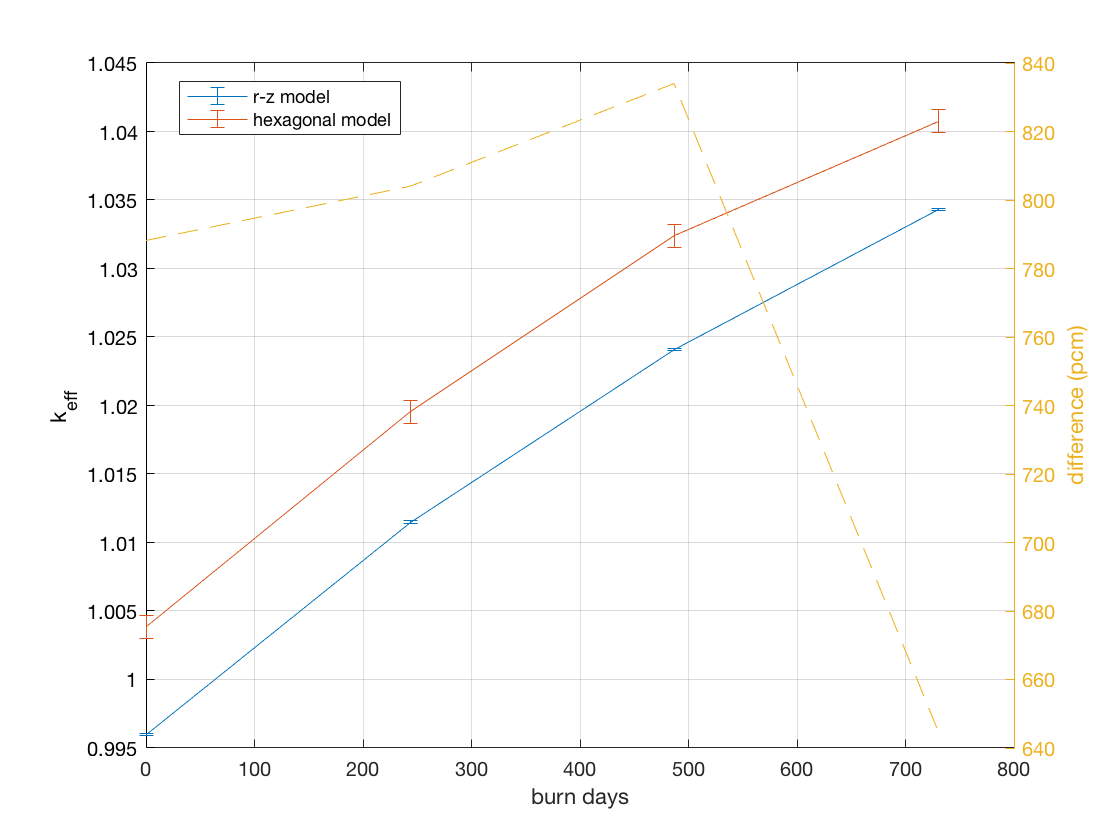
\includegraphics[width=10cm]{keff}
%\centering
%\caption{Evolution of $k_{eff}$ over the equilibrium cycle as calculated with both the hexagonal and the simplified r-z transport models.}
%\label{fig:keff}
%\end{figure}

%%%%%%%%%%%%%%%%%%%%%%%%%%%%%%%%%%%%%%%%%%%%%%%%%%%%%%%%%%%%%%%%%%%%%%%
\section{Orificing}

For this study, it is assumed that the orificing is made integral to the gridplate, as opposed to having orifices attached to the bottom of each assembly.
This is done to simplify the difficult task of designing orifices for B\&B cores with assemblies that vary in power by multiple orders of magnitude over their residence times in the core.
Doing this also allows for the plant thermodynamic cycle to be more efficient and consistent, as the core outlet temperature can be kept at the desired value more easily.
If the orificing is executed within each specific assembly, at various points the assembly will be very under- or over-cooled.
By making the orifices integral to the gridplate, these inefficiencies can be avoided.
The obvious difficulty with gridplate orificing is that it complicates the design of startup cycles, where the power profile could potentially look drastically different than the equilibrium power profile.
For this study, such complications are not considered and it is assumed that this orifice strategy does not interfere with the reactor startup cycles.

With the power profile established, an orificing strategy for the core can then be designed.
In order to accomplish this task, the optimization code ORFS \cite{ORFS} is utilized to obtain an orificing that conforms to the following constraints:

\begin{enumerate}
\item $T_{out, max} \leq 655$ C
\item $T_{out, mean} = 510 \pm 5$ C
\item $\Delta p_{max} \leq 1$ MPa
\item $v_{max} \leq 12$ m/s
\item $\Delta T_{out, adjacent} \leq 70$ C
\end{enumerate}

To gather the assemblies into orifice groups, logarithmic spacing into 28 groups is utilized.
With fewer groups, the problem becomes infeasible due to the constraint on temperature difference between adjacent assemblies.
In reality, with differences of up to 60 C between adjacent assemblies, significant heat transfer will occur between the assemblies causing the assembly outlet temperatures to be somewhat of an average, although this is not accounted for in the ORFS optimization process. 
An additional aspect that is not accounted for is that the material composition within each assembly used to determine the power profile is currently set to be constant within all assemblies of a batch.
This leads to a steep, sudden transition in isotopics between adjacent assemblies that are in different batches.
In the actual equilibrium cycle, the isotopics will likely transition more smoothly between adjacent assemblies due to the smooth neutron flux profile.
Both of these aspects lead to the current optimization constraints being more restrictive than the actual physics will dictate.
A relaxation of these constraints could lead to the problem being feasible for a smaller number of orifice groups or to smaller temperature gradients between adjacent assemblies, but this issue is not investigated further due to the fact that current results for orifice groupings are in line with the goals of other reactor designs \cite{terrapower}.

After feeding the power profile and aforementioned constraints to ORFS, the code attempts to minimize the variance in outlet coolant temperatures by allocating flow to each assembly, including control and reflector assemblies.
The general results of this optimization procedure are given in Figures \ref{fig:BnB_0_temp}-\ref{fig:BnB_3_temp} and Table \ref{tab:orificing}.

\begin{figure}[h!]
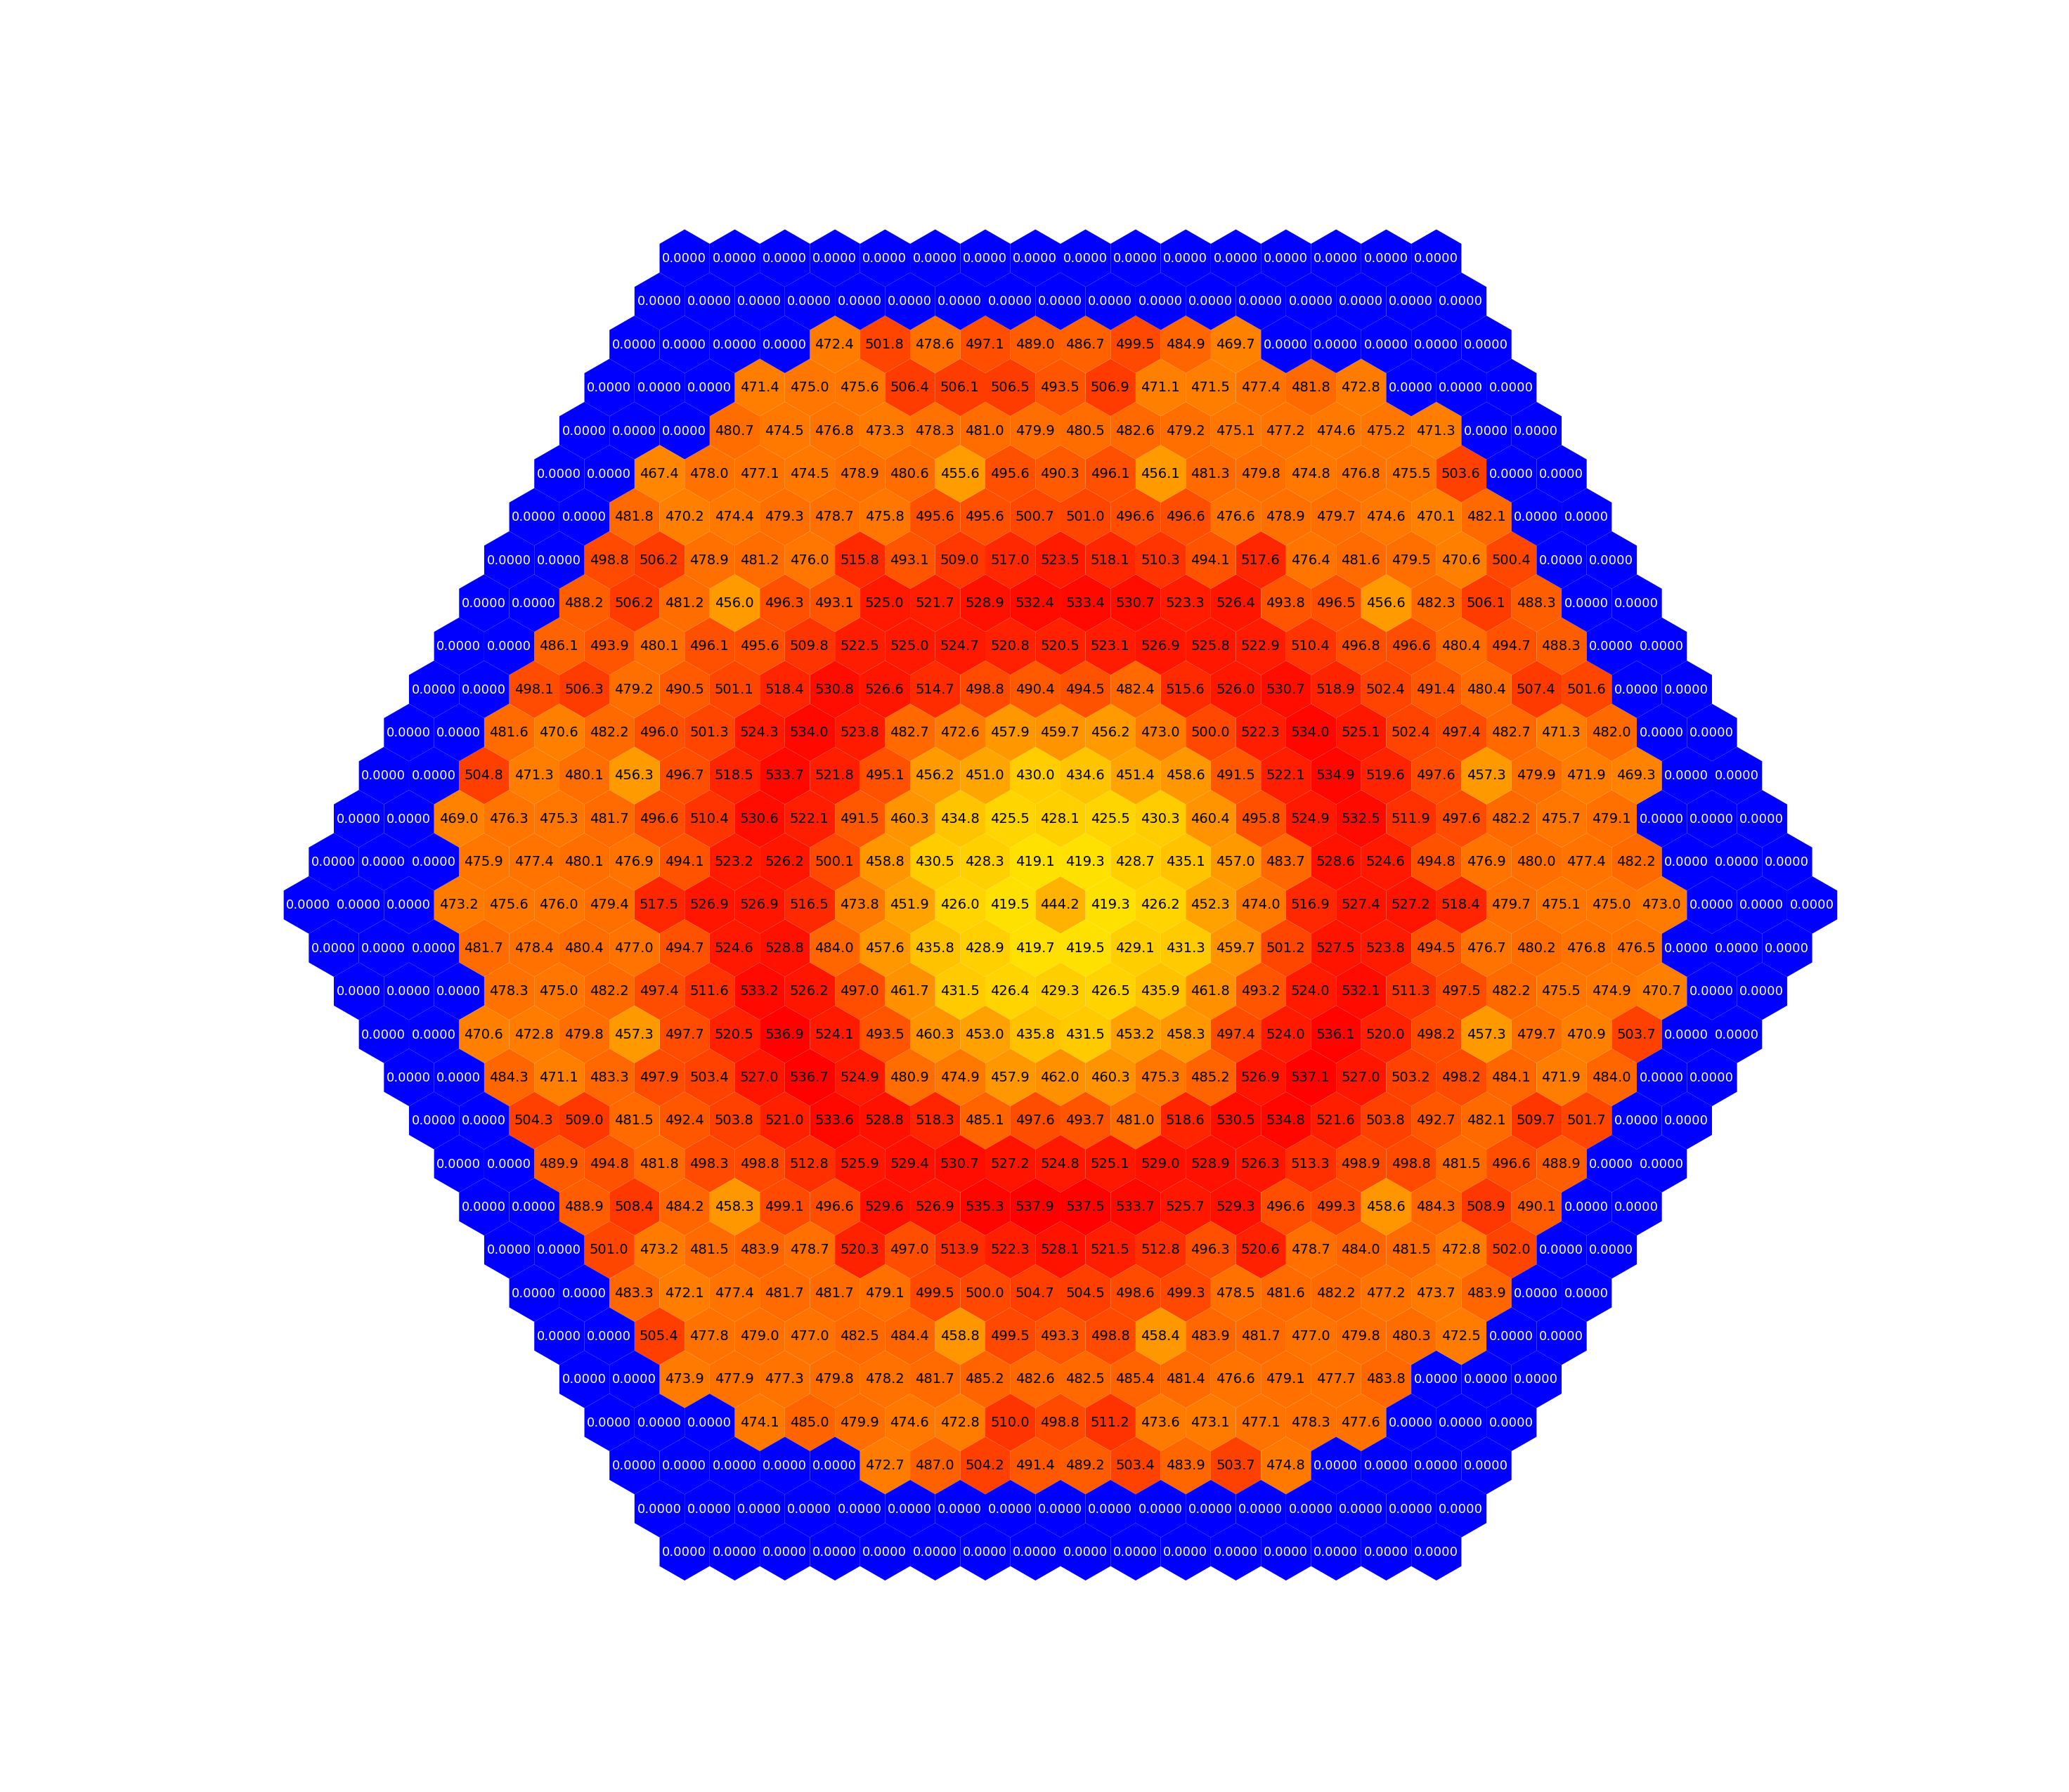
\includegraphics[width=16cm]{BnB_0_temp}
\centering
\caption{Temperature profile of the 3500 MWth B\&B core at BOEC. Temperatures are listed in C and assemblies shown in dark blue are not considered in the optimization due to their extremely low power.}
\label{fig:BnB_0_temp}
\end{figure}

\begin{figure}[h!]
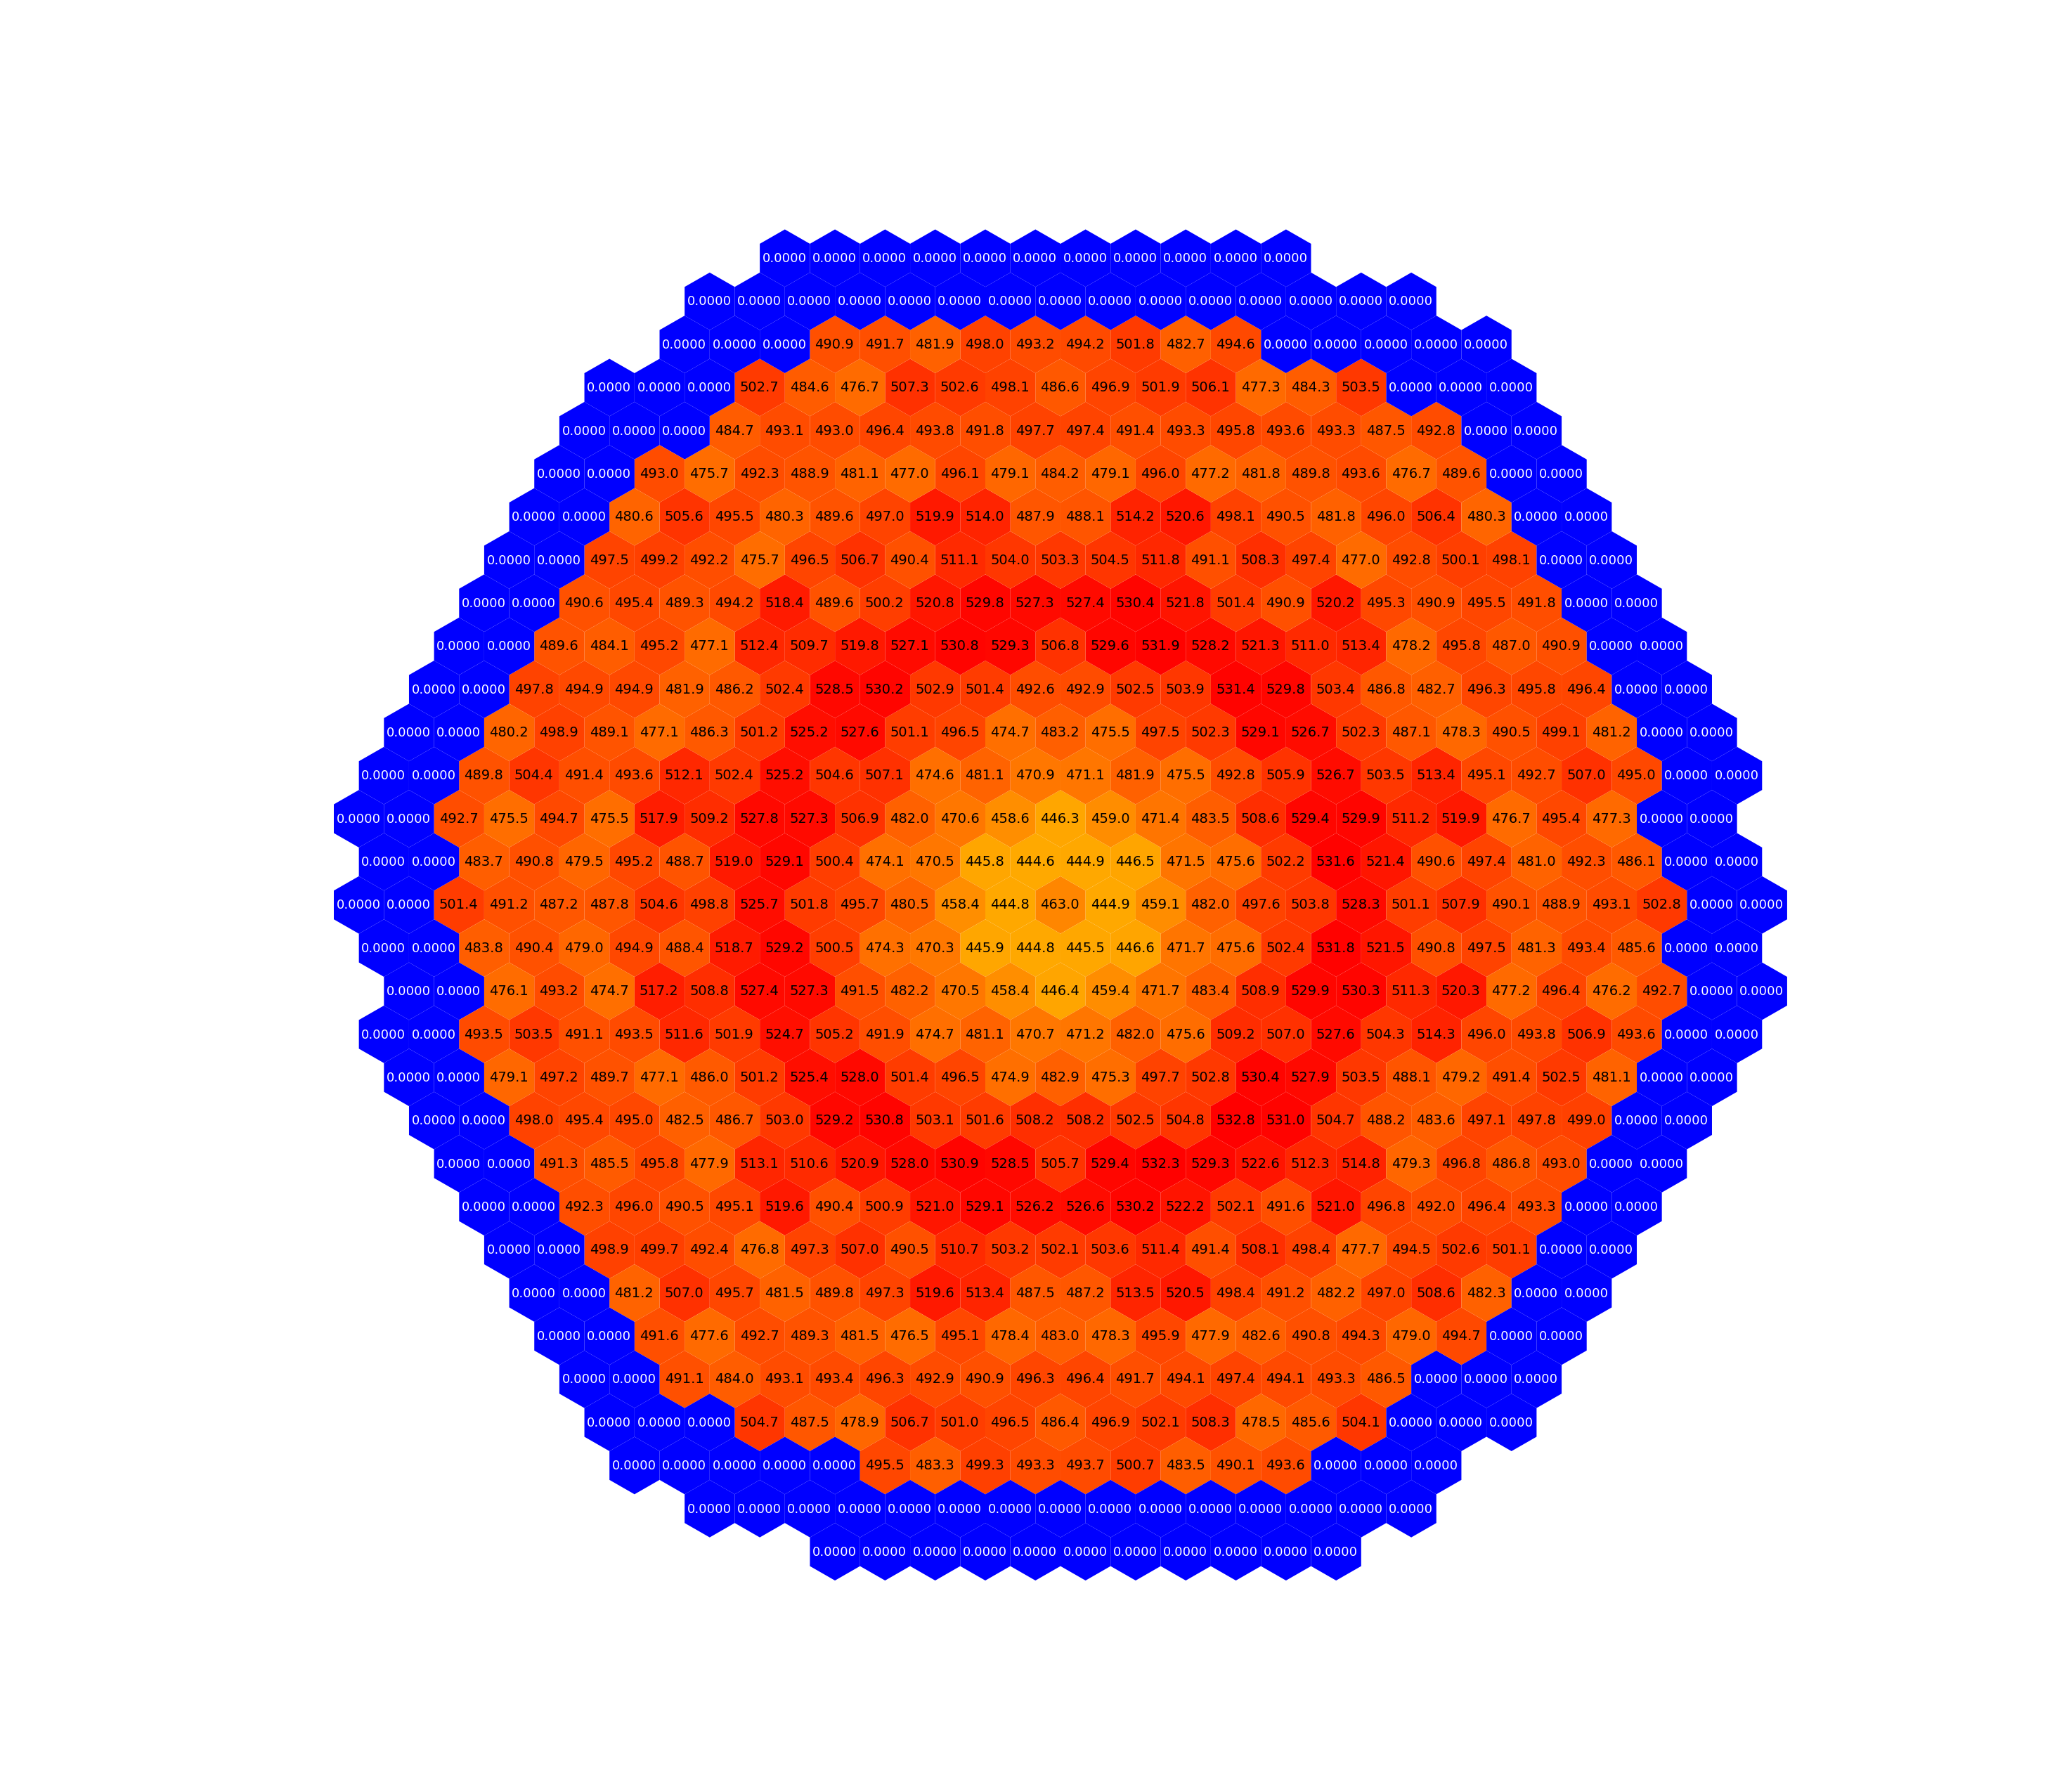
\includegraphics[width=16cm]{BnB_1_temp}
\centering
\caption{Temperature profile of the 3500 MWth B\&B core at MOEC1. Temperatures are listed in C and assemblies shown in dark blue are not considered in the optimization due to their extremely low power.}
\label{fig:BnB_1_temp}
\end{figure}

\begin{figure}[h!]
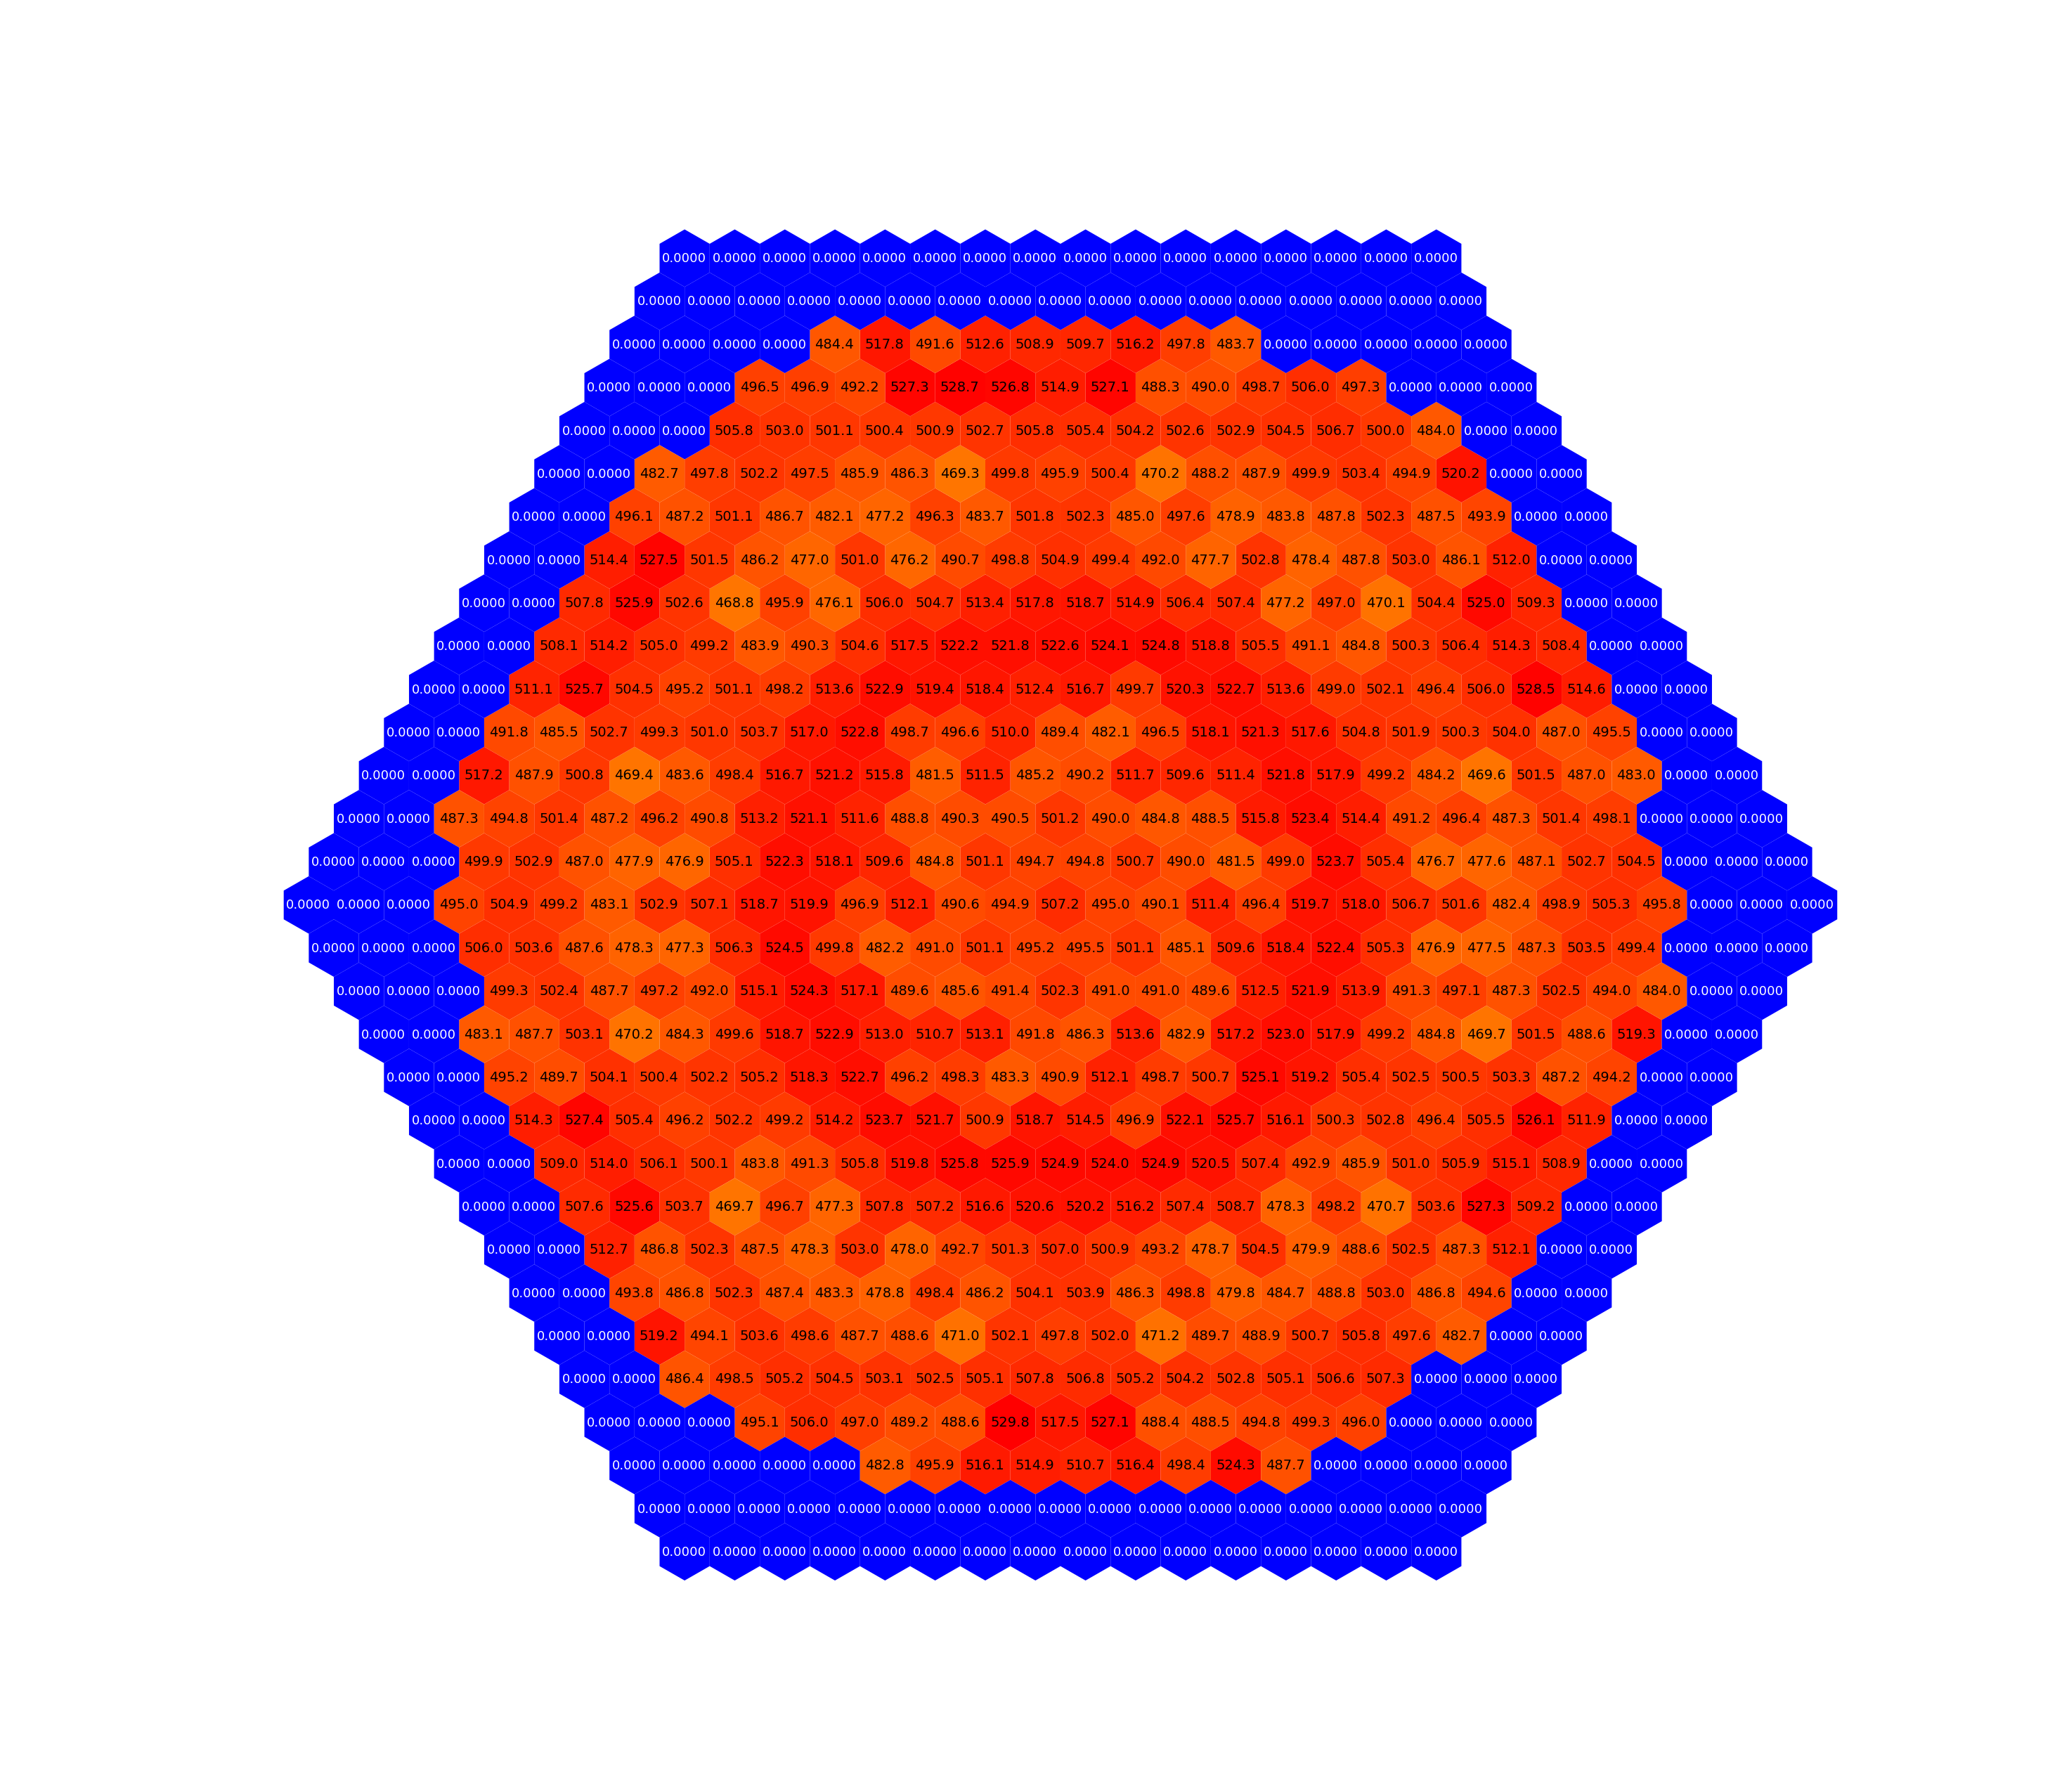
\includegraphics[width=16cm]{BnB_2_temp}
\centering
\caption{Temperature profile of the 3500 MWth B\&B core at MOEC2. Temperatures are listed in C and assemblies shown in dark blue are not considered in the optimization due to their extremely low power.}
\label{fig:BnB_2_temp}
\end{figure}

\begin{figure}[h!]
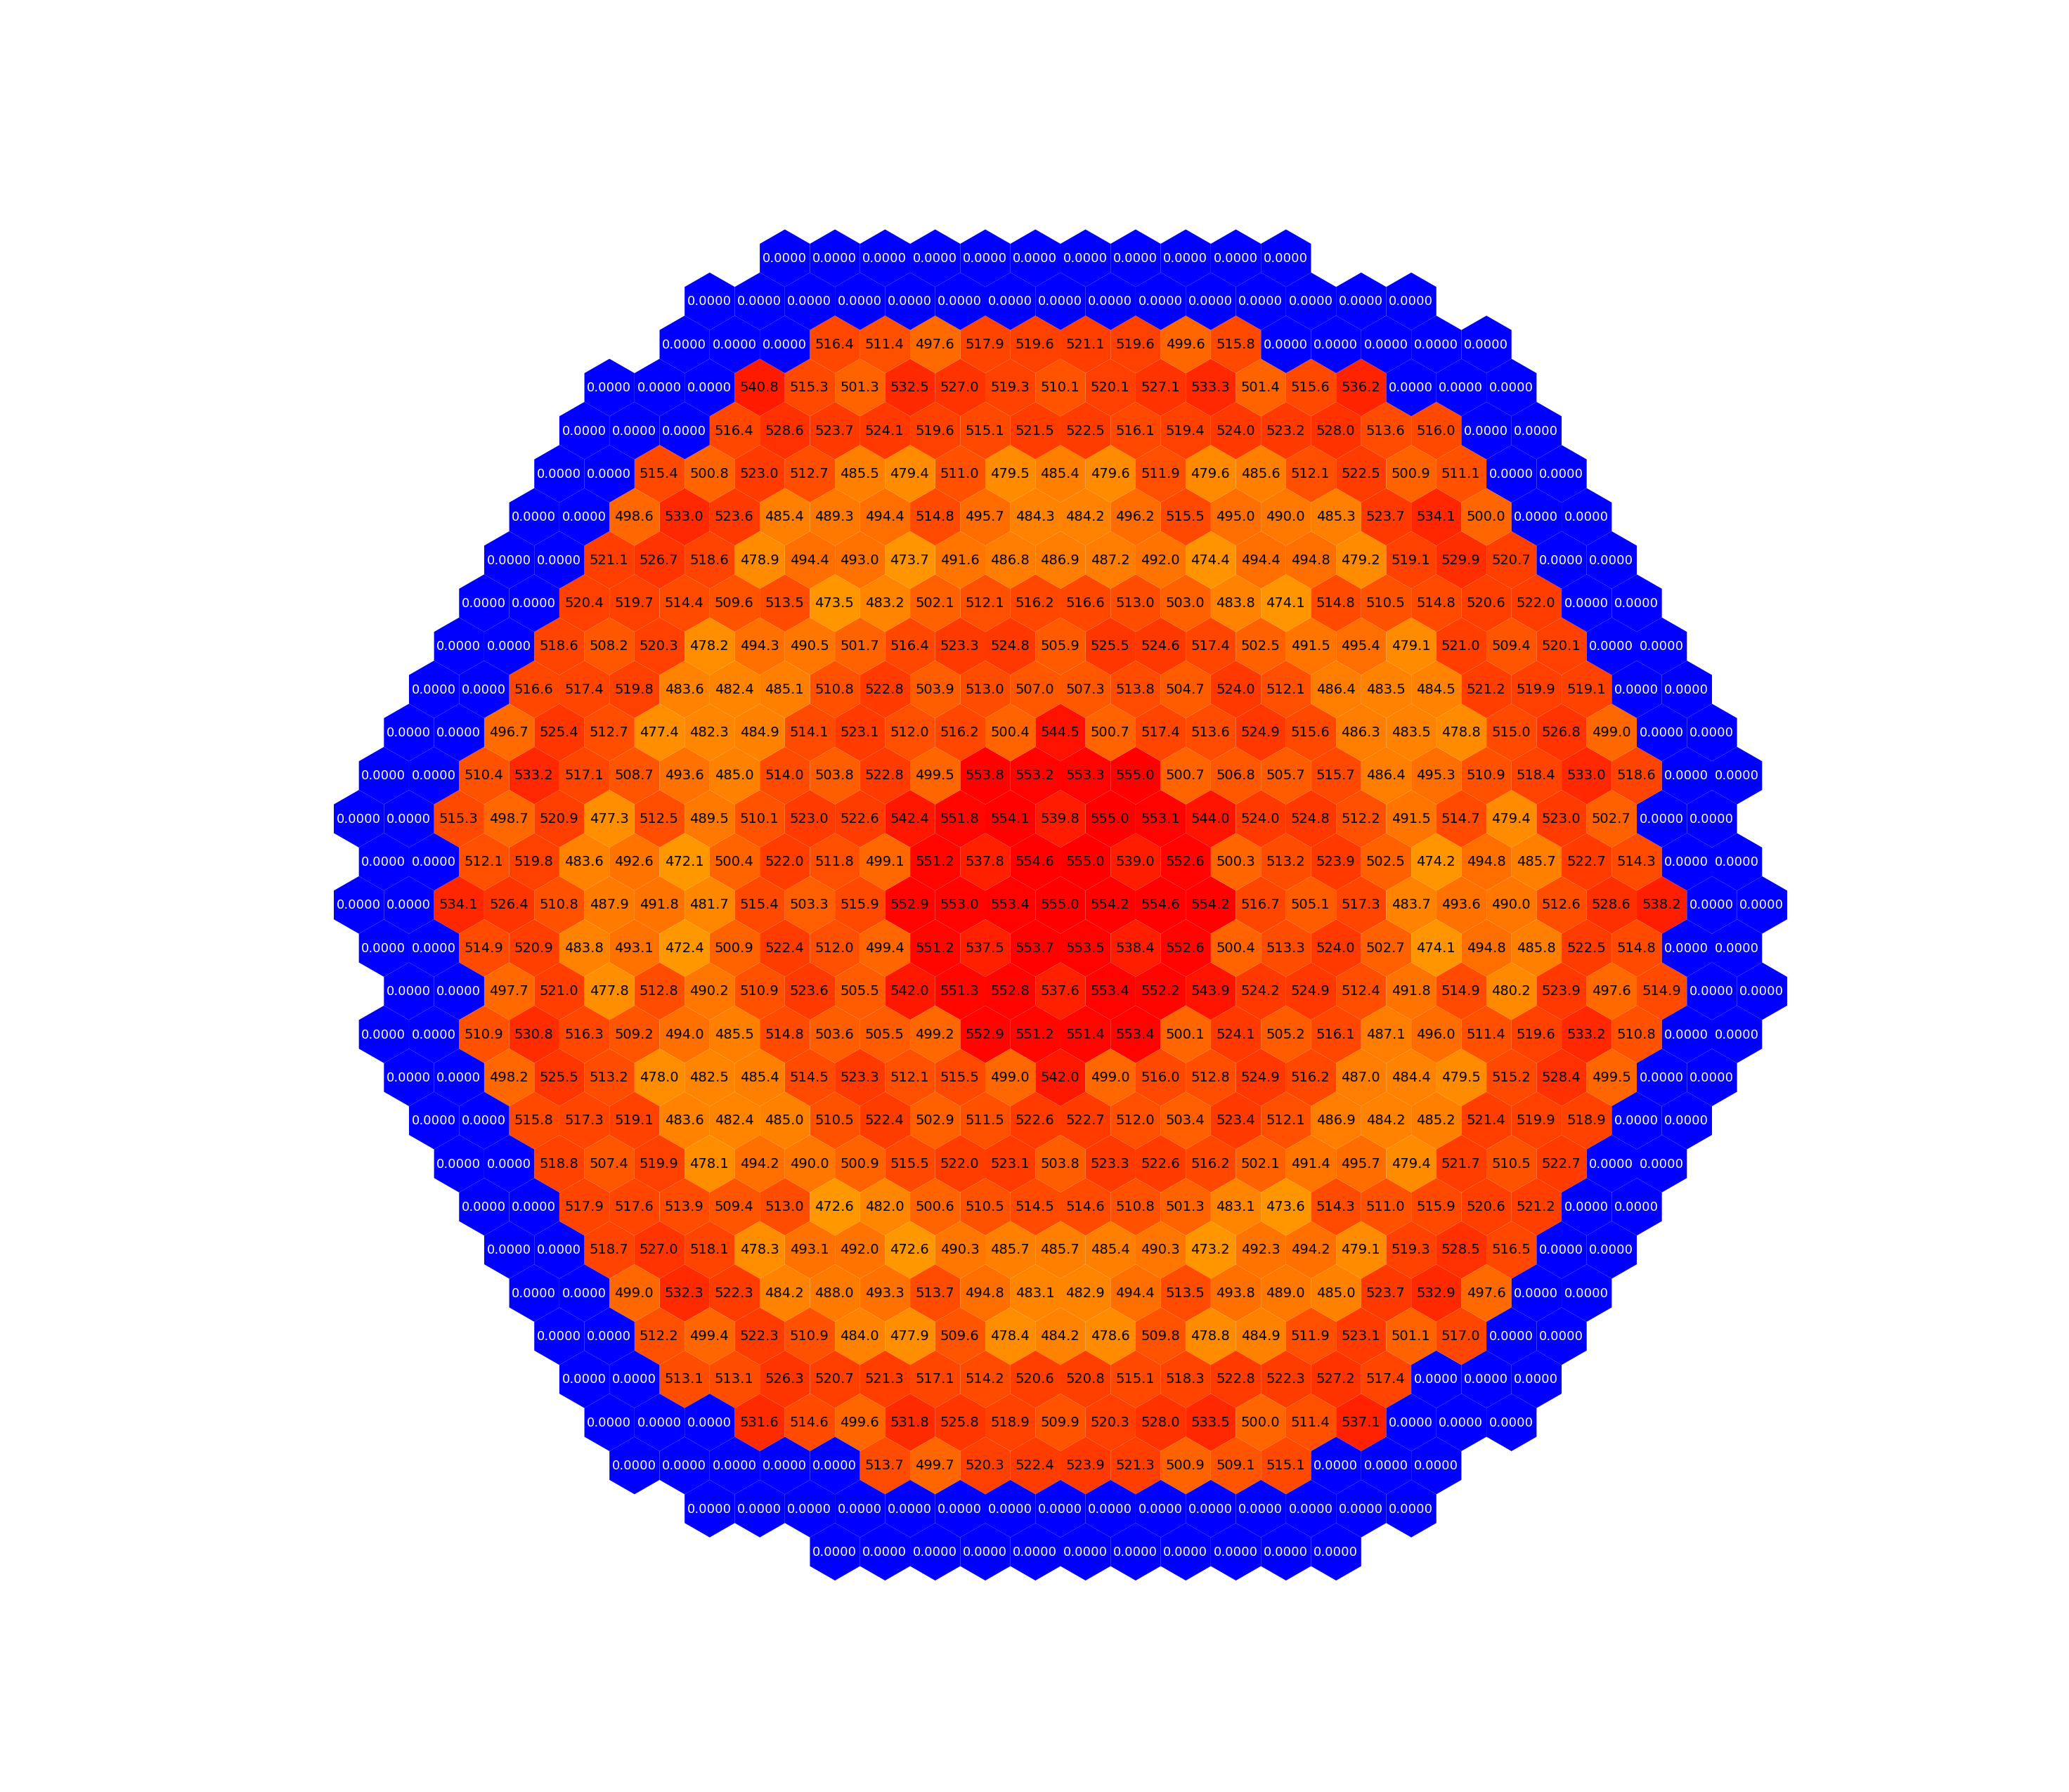
\includegraphics[width=16cm]{BnB_3_temp}
\centering
\caption{Temperature profile of the 3500 MWth B\&B core at EOEC. Temperatures are listed in C and assemblies shown in dark blue are not considered in the optimization due to their extremely low power.}
\label{fig:BnB_3_temp}
\end{figure}

\begin{table}[]
\centering
\caption{General temperature characteristics of the 3500 MWth B\&B core determined with 28 logarithmically-spaced orifice groups from the ORFS code.}
\label{tab:orificing}
\begin{tabular}{@{}ccccc@{}}
\toprule
Burn Step & Burn Time (days) & max $T_{out}$ (C) & $T_{out,mixed}$ (C) & max $\Delta T_{out, adjacent}$ (C) \\ \midrule
BOEC      & 0                & 537.9             & 505.1               & 40                                 \\
MOEC1     & 243.3            & 528.4             & 505.1               & 30                                 \\
MOEC2     & 486.6            & 529.8             & 505.0               & 25                                 \\
EOEC      & 730              & 555.0             & 505.0               & 60                                 \\ \bottomrule
\end{tabular}
\end{table}

The maximum outlet temperature as calculated from the simple model in ORFS occurs at the EOEC in an assembly adjacent to the central assembly.
In the optimization, the constraint on maximum outlet temperature at EOEC is tight, along with the constraints on the lower bound for the mean outlet temperature for all burn steps.
None of the constraints are tight at any point during the equilibrium cycle.
Therefore, the overall limiting period of the burn is at EOEC, and this is the core state that should be studied the most heavily during the safety analysis. 
The peak inner cladding temperature, which should be used as the limiting factor for the orifice determination in a metal fueled core, has not yet been accurately quantified.
It is planned that this will be quantified during the actual safety analysis with SAS, and if required, the orificing will be iterated to achieve a suitable peak inner clad temperature.

%%%%%%%%%%%%%%%%%%%%%%%%%%%%%%%%%%%%%%%%%%%%%%%%%%%%%%%%%%%%%%%%%%%%%%%
\section{SAS channel grouping}

After the assembly orificing strategy is determined, the specific modeling of the full core with SAS can be considered.
SAS operates by simulating a limited number of channels, which are multiplied as needed to represent the entire core.
Each channel represents a single subchannel within an assembly.
Therefore, to accurately capture the transient response of the reactor, assemblies need to be bundled together into appropriate groups, and then the average of these groups is simulated.
In a typical SFR core with inner, middle, and outer core zones denoted by different enrichment levels, the grouping is often done along those lines.
This is logical because the power, reactivity coefficients, and flow allocation generally fall nicely into groups which align with the enrichment level.
In addition to the groups corresponding to the enrichment zones, typically a separate channel will be dedicated to the assembly with the peak power-to-flow ratio so that limiting transient temperatures can be quantified, and another channel will be used for modeling the reflector assemblies, which account for a substantial portion of the core flow even though they are low in power.

In the B\&B core of interest to this study, the situation is not quite as clear-cut.
The many batches across the core provides more of a smooth gradient in material compositions than would be seen in a core with just a few batches.
Furthermore, many of the batches, particularly towards the periphery, have disjoint groups of assemblies, and therefore may transfer heat very effectively between multiple batches, which can complicate the SAS model development.
Therefore, the approach taken for grouping assemblies into representative channels for SAS modeling is to limit the number of representative channels to less than the number of batches by grouping batches of similar power and temperature together.

This can be accomplished by examining the outlet temperature profile for the limiting burn step (i.e. EOEC) plotted in Figure \ref{fig:BnB_3_temp} and trying to line this up with a combination of the batches plotted in Figure \ref{fig:BnB_layout}.
In Figure \ref{fig:BnB_3_temp}, a few rough temperature clusters can be seen with a central high-power high-temperature zone in the first few rings, a high-power medium-temperature zone in the next couple rings, a high-power low-temperature zone in the next few rings, and a low-power low-temperature zone in the remaining fueled assemblies.
Another zone is then allocated for reflector, shield, and control assemblies since they contain no fissionable material.
Finally, the assembly with the highest outlet temperature is chosen to as a final group.
(It should be noted that this peak assembly could be any of those surrounding the central assembly position, as all of them should have the same power and flow due to the 1/6 core symmetry. They do not have the same exact power due simply to monte carlo statistics.)

Based upon the observed temperature profile and in consultation with the batch layout, the assemblies are grouped into representative channels as shown in Figure \ref{fig:BnB_SAS_layout}.
In this chosen grouping, each batch is wholly contained within a channel, which greatly simplifies the process of determining averaged reactivity coefficients for each representative channel later on.

\begin{figure}[h!]
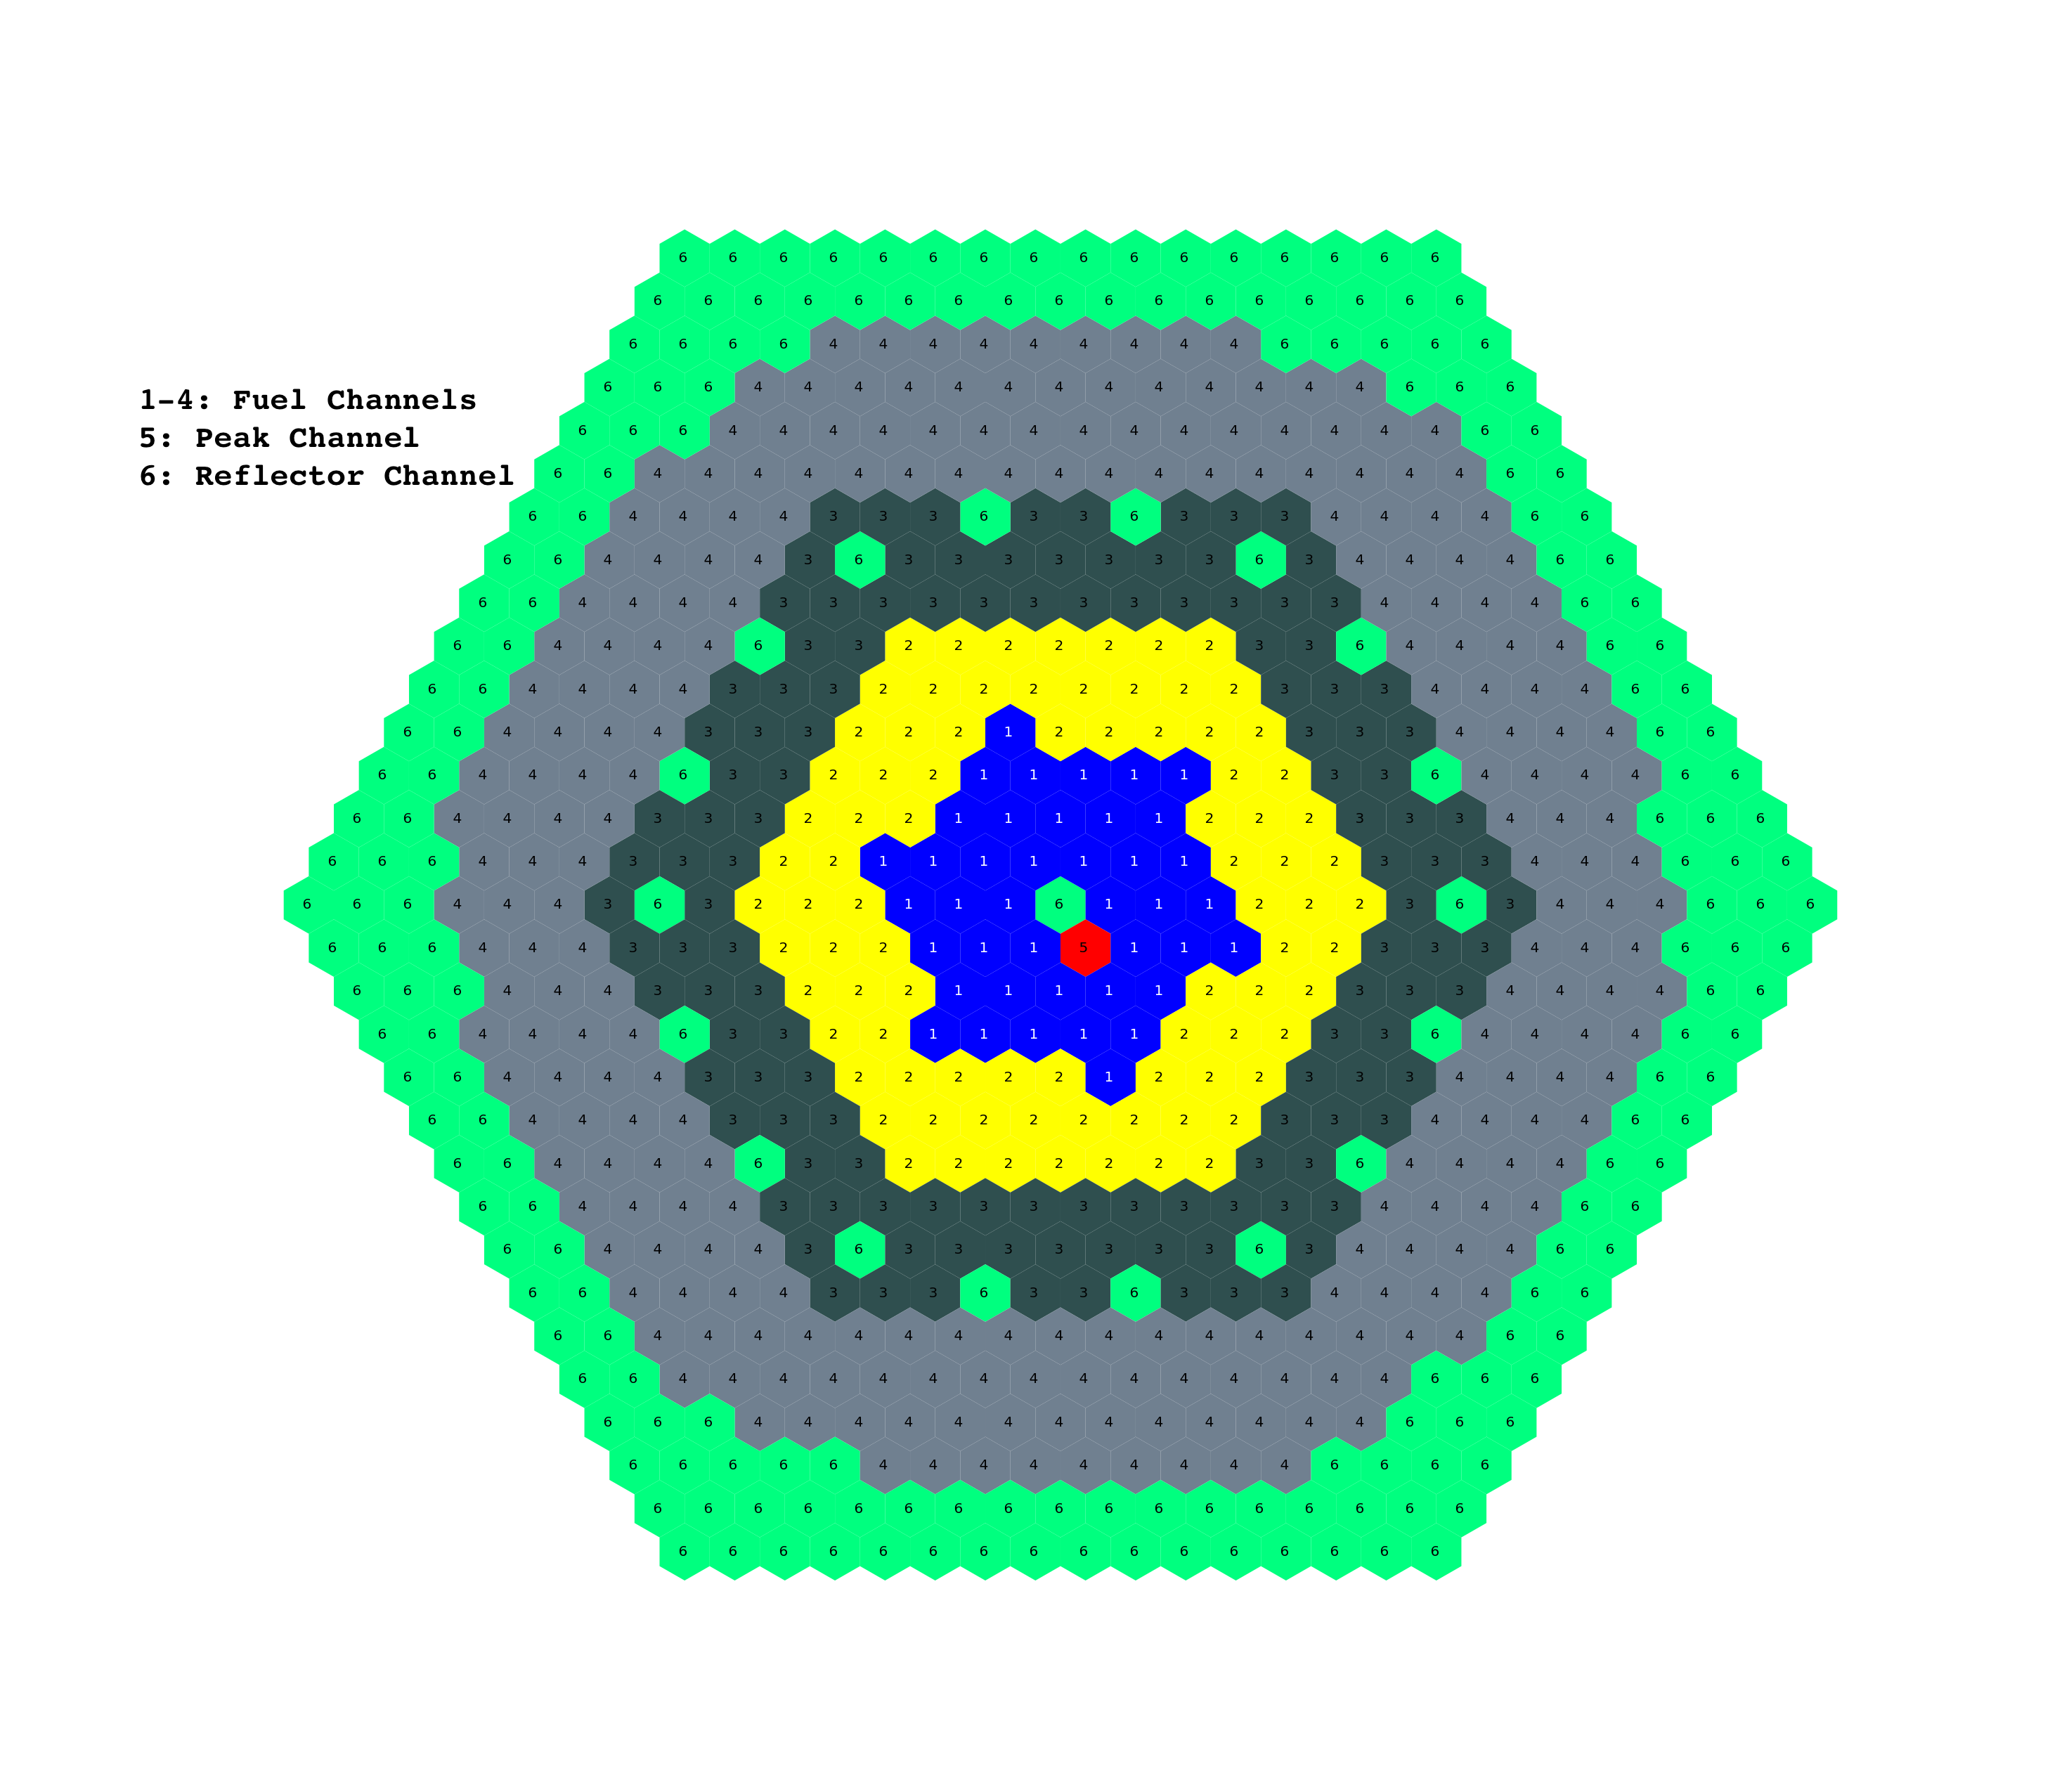
\includegraphics[width=16cm]{BnB_SAS_layout}
\centering
\caption{Representative groups used to model the 3500 MWth B\&B core in SAS.}
\label{fig:BnB_SAS_layout}
\end{figure}

\begin{thebibliography}{9}

\bibitem{Qvist_3D}
S. Qvist, J. Hou, E. Greenspan, "Design and performance of 2D and 3D-shuffled breed-and-burn cores," Annals of Nuclear Energy, Vol 85, 2015.

\bibitem{serpent}
Lepp�nen, J., et al. (2015) "The Serpent Monte Carlo code: Status, development and applications in 2013." Ann. Nucl. Energy, 82 (2015) 142-150. 

\bibitem{SAS}
J. E. Cahalan and T. H. Fanning, The SAS4A/SASSYS-1 Safety Analysis Code System, Argonne National Laboratory.

\bibitem{heidet_thesis}
F. Heidet, "Maximum Fuel Utilization in Advanced Fast Reactors without Actinides Separation," PhD Thesis, University of California Berkeley, 2010. Pgs 75-77.

\bibitem{ADOPT}
S. Qvist, E. Greenspan, "The ADOPT code for automated fast reactor core design," Annals of Nuclear Energy, Vol 71, 2014.

\bibitem{mocdown}
J. E. Seifried, P. M. Gorman, J. L. Vujic, and E. Greenspan. Accelerated Equilibrium Core Composition Search Using a New MCNP-Based Simulator. Proceedings of the SNA\&MC 2013 conference, Paris, France, October, 2013.

\bibitem{endf}
M. B. Chadwick, M. Herman, P. Oblozinsky, et al., "ENDF/B-VII.1 nuclear data for science and technology: Cross sections, covariances, fission product yields and decay data", Nuclear Data Sheets, 112(12):2887-2996 (2011).

\bibitem{mcplib}
$https://mcnp.lanl.gov/BUGS/la-ur-12-00018_mcw.pdf$

\bibitem{ORFS}
C. Keckler, "A Simplified Model for Optimal Assembly Orificing in an SFR through Convex Optimization," Internal report, 2017.

\bibitem{terrapower}
P. Hejzlar et al., "Terrapower, LLC Traveling Wave Reactor Development Program Overview," Nuclear Engineering and Technology, Vol 45, 2013.

\end{thebibliography}

\end{document}